%&latex
\chapter{A Protein Structure Database}
\label{chapter:database}

\begin{quote}
``Chance favors the prepared mind.'' \\
--- \textit{Louis Pasteur}
\end{quote}

\section{Introduction}

The Protein Data Bank\cite{NATIVE:PDB:A,NATIVE:PDB:B,NATIVE:PDB:C,NATIVE:PDB:D} (PDB) is a large database of  experimentally derived protein structures, which at the time of writing contains 43,045 entries (table \ref{table:db:pdb}). There is significant redundancy within the PDB, such as structures of single-point mutants and multiple versions of a given protein in complex with different ligands.  In order to perform any meaningful statistical analysis on the sequence-structure relationships within the PDB, a non-redundant set is required.

Critical investigation of protein modelling methodologies requires such an idealised data set for the purpose of calibration and testing. To this end, two databases have been created in this work. The primary database is a subset of the entire PDB and is intended to be a representative set of all known protein structures to date. This \dataset\ facilitates statistical analyses of protein structure and acts as a \testset\ for protein modelling. Derived
from this database is a representative set of medium to long length loop structures for use in
the calibration and benchmarking of loop modelling methods.

\begin{table}[htbp]

\begin{center}
\begin{small}        
\begin{tabular}{+c^c^c^c^c^c}

\toprule 
\rowstyle{\bfseries} Experimental & \multirow{2}{*}{Proteins} & Nucleic Acids & Protein/NA  & \multirow{2}{*}{Other} & \multirow{2}{*}{Total} \\ 
\rowstyle{\bfseries} Method       &          & (NA)          & Complexes &       & \\
\midrule
   X-ray    & 34,017 &   963 &  1,570 & 28 & 36,578 \\
   NMR      &  5,346 &   753 &    129 &  7 &  6,235 \\
   EM       &     97 &    10 &     38 &  0 &    145 \\
   Other    &     80 &     4 &      3 &  0 &     87 \\
\midrule
   Total    & 39,540 & 1,730 &  1,740 & 35 & 43,045 \\
\bottomrule

\end{tabular}
\end{small}
\end{center}

\caption{PDB holdings breakdown: 27\superscript{th} April 2007.}
\label{table:db:pdb}

\end{table}


\section{Caveats of Atomic 3D Structure}
\label{DB:NativeProbs}


In nature, protein structures are highly dynamic and heterogenous entities in aqueous solvent\cite{NATIVE:Frau1991}. They are known to show
anisotropic motion and exhibit discrete conformational sub-states, the dynamics of
which can be functionally important\cite{NATIVE:DePristo2004}.
Surface loops, which have the least contact with the rest of the fold can exhibit structural transitions.
These include both rare transitions between competing isoenergetic minima and large structural fluctuations around a single minimum, termed static and  dynamic disorder respectively.

Traditionally, it is usual to represent proteins as a single structure unless strong evidence exists to support specific
multiple conformational sub-states. The majority of reliable publicly available experimental data is therefore published
as single structural representations. It is unfortunately not usual to quantify perceived uncertainty by showing valid conformational sub-states. In more recent times there have been
calls to halt this trend, by rejecting the practise of using single models,
in favour of representative ensembles\cite{NATIVE:Terwilliger2006}. This would particularity benefit models with regions of low certainty and would provide greater clarity for applications such as drug docking
and surface loop prediction.

For the time being, however, PDB \subsets\ can only be derived from the data contained
within the PDB itself. This work will therefore utilise a single native state
for each polypeptide chain, with the caveat that only those where there is high
structural certainty should be included. This practise
also simplifies structural analysis as it would be difficult to score
a given model structure against an entire ensemble.  \subsection{ NMR Spectroscopy for Proteins}

NMR, or Nuclear  Magnetic Resonance, has been used successfully to determine around 13.5\% of the PDB entries to atomic detail. Briefly, in NMR, a concentrated protein solution is prepared and usually multiple complementary NMR spectra are obtained. From these spectra, resonances are assigned and a series of spatial constraints are generated.
These constraints include distance restraints from NOESY spectra, angle constraints from coupling constants and orientation restraints from residual dipolar coupling.
From the satisfaction of this constraint matrix, an ensemble of candidate structures can be generated
and validated. Figure \ref{fig:db:nmr} shows PDB entry 1A57 as a typical example of an NMR structure.


\begin{figure}[p]
  \begin{center}
  
  \subfigure[The Full Structural Ensemble]{\scalebox{0.65}{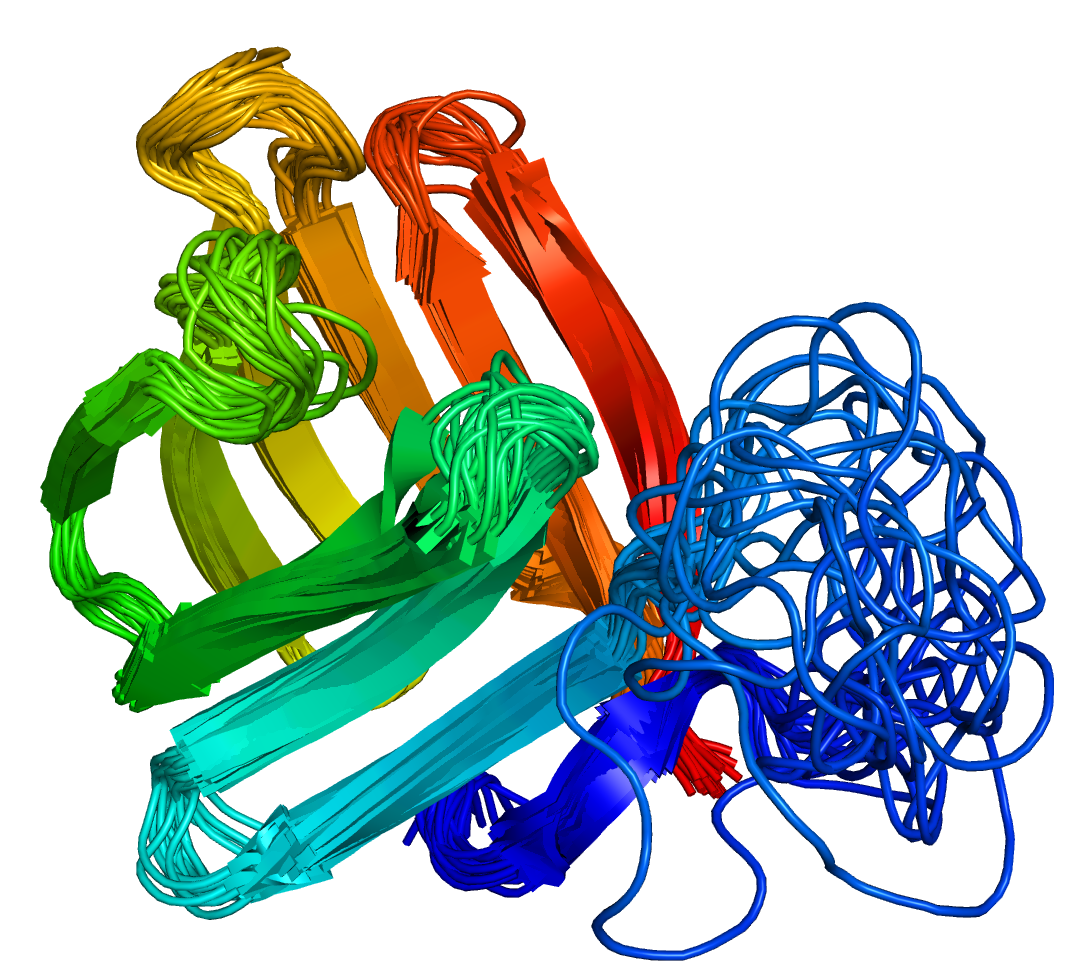
\includegraphics[width=1.0\textwidth]{04-Database/nmr/nmr_ensemble.png}}}
  \label{fig:db:nmr:a}
  \subfigure[Structural variation: Protein core \sidechains\ (Models 1-6 residues 33-36)]{\scalebox{0.75}{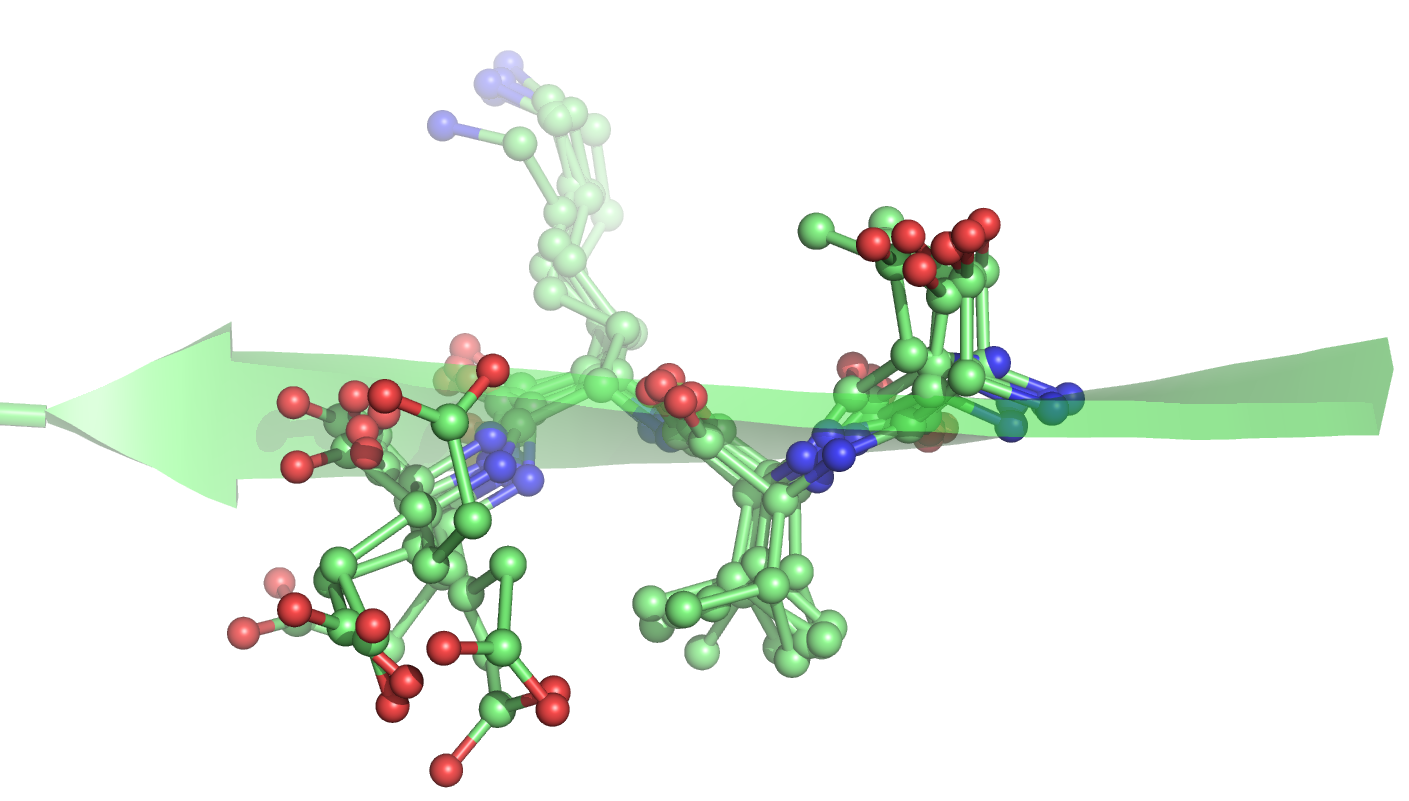
\includegraphics[width=1.0\textwidth]{04-Database/nmr/nmr_core.png}}}
   \subfigure[Structural variation: Surface \mainchain\ (Models 1-8, residues 98-111)]{\scalebox{0.75}{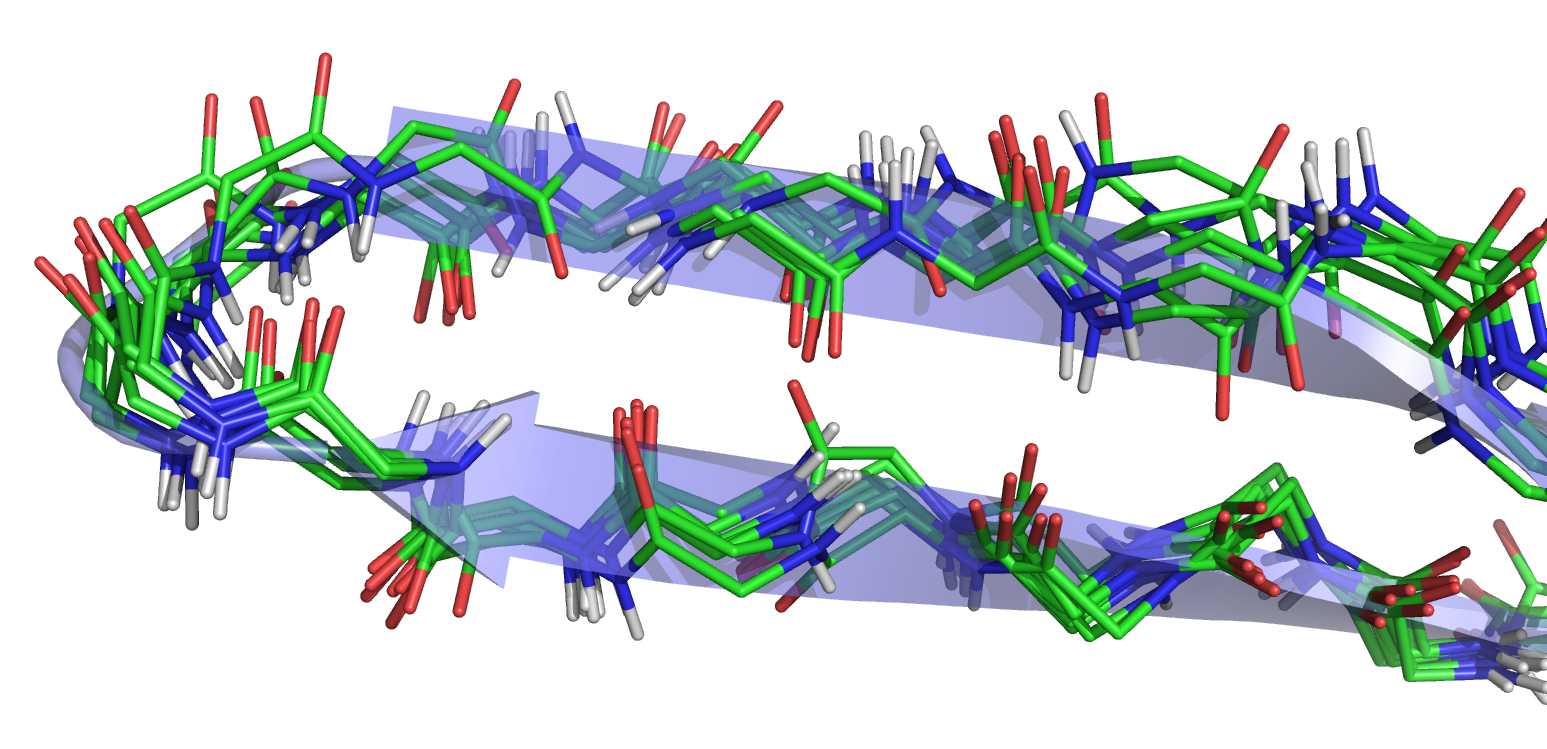
\includegraphics[width=1.0\textwidth]{04-Database/nmr/nmr_backbone.png}}}
      
    \caption[NMR Structure 1A57]{NMR structure 1A57, which contains 20 models.}
    \label{fig:db:nmr}
  \end{center}
\end{figure}



Originally most NMR structures were solved using metric matrix distance geometry (\mbox{\textsc{Diana}\cite{METHOD:DIANA:A,METHOD:DIANA:B}}), however current state of the art programs (\eg\ \mbox{\textsc{Xplor}\cite{NATIVE:XPLOR}}, \mbox{\textsc{Dyana}\cite{METHOD:DYANA:A,METHOD:DYANA:B}}) employ a combination of distance geometry and restrained molecular dynamics
(MD). MD has also been used in similar contexts such as protein model production from limited constraint sets\cite{METHOD:van94} and homology structure refinement\cite{METHOD:Fan2004}. Other NMR techniques have utilised conjugate gradient minimisation, molecular dynamics and simulated annealing in combination\cite{METHOD:Clo86}. There are however difficulties with the use of NMR structures within an idealised
PDB \mbox{sub-set}: 

\begin{enumerate} \isep
\item 
NMR data does not provide information about bonded
interactions, such as bond lengths and angles -- only non-bonded interactions are defined. The NMR restraint list therefore must included similar harmonic bond, angle and torsion terms to those in molecular mechanics \forcefields.
This in turn introduces structural bias if NMR derived information is used for benchmarking models produced using similar \forcefield\ terms. 

\item Most NMR structures are published as an \emph{ensemble} of valid structural states which satisfy the available restraints. There is however a large variation in the number of presented
structures in the ensemble from 1 up to 50, although most have around 20, complicating analysis of the ensemble. Some models are even presented as a single energy-minimised average
of all generated structural models, meaning that the information contained
within the ensemble is lost.

\item Following the satisfaction of the constraint matrix, there can still be large
deviations within the structural ensemble. This is exemplified by figures \ref{fig:db:nmr}-b
and \ref{fig:db:nmr}-c which show that both core \sidechains\ and surface \mainchain\
structures show significant deviations within the ensemble. 

\item Only protein segments for which restraints are present will have defined structure, often meaning that the N and C-termini and some more flexible surface loops will either have poor or no
structural definition in the final model \mbox{(figure \ref{fig:db:nmr}-a, blue C-terminal structure).} There is  no single standard for per-atom or per-residue quantification of structural certainty. Critically, therefore, such flexible regions are often present within the structure definition file, but sometimes have little quantification
of their certainty, making interpretation against
model structures difficult. Such scores could potentially be derived from
the structural ensemble and the original restraint list; The restraint list itself, however, is sometimes not published or of variable format. 

\end{enumerate}



Overall these facts make NMR data unsuitable for the work described in this
dissertation.





\subsection{X-Ray Crystallography}

Structures derived via \xray\ crystallography are currently the best standard available for benchmarking protein models. The majority are presented as single averaged structures and modelled with Gaussian, isotropic thermal motion. Each structure is an iteratively refined best fit of a structural model to available \xray\ diffraction data. There is, however, some debate about just how accurate and representative these structures are.
Automated refinement methods are in development\cite{NATIVE:DePristo2005,NATIVE:Adams2004}, but for the foreseeable future the majority of the PDB will have been produced using traditional crystallographic refinement, which is both labour intensive and directed by human judgement. 

Over 90\% of \xray\ structures diffract to $>$1.6\AA\ resolution, at the level where heterogeneity is hard to identify and model. It is thought that disregard for structural heterogeneity could cause difficulties in structural determination, as multiple isotropic models can explain the diffraction data equally well\cite{NATIVE:DePristo2004}.
More importantly, significant differences between these models shows that the accuracy of \xray\
crystallography for lower resolution structures is over-estimated as a whole.

Observed diffraction intensities are averaged over both space and time. Crystallographic B-factors, also known as temperature factors, are a measure of thermal motion of each atom and hence its structural
order.  If a group or single atom simultaneously occupies two isoenergetic positions within the unit cell, then they are said to have fractional occupancy; that is to say their position within the unit
cell is not constant. Selection of structures for a reduced PDB \jsubset\
should, therefore, take these two parameters into account.  

In a recent work comparing the 25 available non-isomorphous crystal forms of T4 lysozyme\cite{NATIVE:Zhang2004},
it was shown that varying crystal contacts perturb backbone atom positions by between 0.2\AA\ and 0.5\AA. Interestingly, the thermal factors of \sidechain\ atoms in individual structures correlate well with  the averaged values, whereas those for backbone atoms do not. This suggests that \xray\ structure thermal values are representative of \sidechain\ motion in solution, but not of backbone motion. This, in turn, shows that in some cases surface backbone conformation can be constrained by the crystal lattice. Such
findings are supported by other work on the effects of crystal packing\cite{METHOD:Plop:Jacobson2002A}.

Studies on the conformational quality of \xray\ structures often focus on
the Ramachandran map. As described in section \ref{section:intro:ramachandran}, the Ramachandran map can be conceptually divided into regions annotated ``allowed'' and ``disallowed'' based
on hard-sphere modelling of the protein \mainchain. This modelling is largely
successful as the bulk of the distribution lies within the allowed regions, however,
there are notable exceptions. These specifically include the disallowed population at $\Phi$ = 60\degree, $\Psi$ = -120\degree\ which is used in a \mbox{type II'} $\beta$-turn \cite{NATIVE:Gunasekaran1996}.
It is also noted that there are a number of \sidechain\ rotameric states which exist in small but structurally defined populations\cite{NATIVE:DePristo2004}. 

It is generally observed that scatter in torsional
distributions is reduced  as resolution improves, signifying an improvement
in overall stereochemical quality\cite{NATIVE:Morris1992}.
Multiple groups have however observed that lower resolution structures actually have a {\em lower} fraction of examples in the ``disallowed'' regions of conformational space. This rather counter intuitive observation suggests that the increased uncertainty in the placement of atoms in lower resolution structures causes the crystallographer to assume conformations lie within a high-propensity
region. In addition to this, other groups observe than many crystallographic structures contain
a small number of significant steric overlaps\cite{METHOD:Plop}; these discrepancies are both attributed
to incomplete model refinement.



\subsection{Summary}

In summary, \xray\ data is currently the best experimental source of  information available. The caveat of using these data is that one
has to assume that a given single high-resolution structure is truly representative of the underlying average  native
ensemble. In order to maximise the
confidence in a given test \dataset\ it is critical that stringent filter criteria for structural quality are applied. Such a filter should utilise per-structure
cutoffs for resolution and R-factor and per-atom cut-offs for temperature-factor and occupancy.
As the ambiguity is reduced by filtering such structures, this should minimise the level of bias introduced by human judgement within the selected \dataset. In terms of protein surface structure prediction, test cases should be chosen where the thermal motion of the surface atoms is minimal within  crystal structure and multiple degenerate \sidechain\ conformations do not exist. 



\section{Standardised PDB Subsets}

The overall aim of the work described in this chapter was to produce a refined subset of the PDB containing only representative polypeptide chains of high quality. Within this \dataset\ all structurally unique protein families should be represented. Several implementations exist in the literature with the ability to create culled PDB subsets by given criteria; all with respective advantages and disadvantages. 

The PDB itself can provide a set of sequences from a given query, culled at either 50\%, 70\%
or 90\% sequence identity; although for the purposes of this work the required single list of all \mbox{high-resolution} chains is not available.

\textsc{Cath}\cite{COMPCHEM:CATH,COMPCHEM:CATH:B} and \textsc{Scop}\cite{COMPCHEM:SCOP,COMPCHEM:SCOP02,COMPCHEM:SCOP04}
are the archetypal domain annotation implementations, providing lists of protein domains, as opposed to entire polypeptide chains. Flat file databases are available with structure quality annotations such as \xray\ resolution. The \textsc{Astral}\cite{NATIVE:ASTRAL} server provides lists of the \textsc{Scop} domain sequences culled at fixed sequence identity cutoffs or E-values derived from \textsc{Blast}\cite{SEQUENCE:BLAST} pairwise alignments. \textsc{Astral} also serves  PDB format files which correspond to the \textsc{Scop} protein domains.

The popular \pdbselect\ server\cite{NATIVE:Hob92,NATIVE:Hob94} had a widespread impact on statistical analysis of the PDB in the literature by providing pre-defined lists of chains with fixed maximum percentage sequence identities. \pdbselect\ follows strict selection criteria to produce its non-redundant protein database. The database is, however, not updated at any regular interval --
at the time of writing the most recent update of the 90\% identity list was March 2006.

\pdbselect\ functions by firstly removing all chains which do not fulfil
the ``Hard-Exclude'' criterion  (table \ref{table:db:pdbselect}).
An efficient sequence alignment algorithm\cite{SEQUENCE:Huang1991} is then utilised in order to group chains by respective pairwise sequence similarity. Chains which cannot be aligned over more than 10 residues are considered to be unrelated, irrespective of their sequence identity. Finally, the ``Soft-Exclude'' criterion is applied to the clustered groups and the best member picked by chain quality, scored using equation \ref{eq:pdbselquality}. 

\begin{table}[tbhp]
\begin{small}\begin{center}
\begin{tabular}{+c^r^p{0.6\textwidth}}
\toprule
\textbf{Exclude} &\multicolumn{2}{l}{\textbf{Description}} \\
\midrule
\textbf{Hard} 
&\textbullet& Length of $<$30 residues \\
&\textbullet& Number of non-standard amino acid residues (including chain breaks) more than 5\% chain length \\
&\textbullet& A resolution $>$3.5\AA \\
&\textbullet& An R-factor $>$30\% \\
&\textbullet& Some chains of known inferior quality \\
\midrule
\textbf{Soft} 
&\textbullet& Number of residues without \sidechain\ coordinates $<$90\% chain length \\
&\textbullet& Number of residues without backbone coordinates is $<$90\% chain length \\
&\textbullet& The content of alanine and glycine $>$40\% chain length \\
&\textbullet& No data on resolution or \mbox{R-factor} are available  \\
&           & (i.e. NMR-structures) \\
\bottomrule
\end{tabular}
\caption{The \pdbselect\ selection criteria.}
\label{table:db:pdbselect}
\end{center}\end{small}
\end{table}


\begin{equation}
\label{eq:pdbselquality}
\mathrm{Quality} = \mathrm{Resolution} + \left( \frac{\mbox{R-factor}}{20} \right)
\end{equation}

The \pdbselect\ implementation has many appealing quality control features, but is inherently not customisable
as it only provides two flat file lists at 25\% and 90\% sequence identity. This is problematic because 25\% would yield too few structures, whereas 90\% will yield highly redundant structural data, even for some surface loops. It also has the disadvantage of not facilitating the complete removal of NMR structures.
 
The \textsc{PDB-ReprDB} server\cite{NATIVE:Noguchi2000} provides a number of the features
which \pdbselect\ lacks, including the ability for the user to set parameters to generate customized lists \mbox{on-the-fly at any sequence identity cut-off}. The server also allows filtering
based on a wide range
of  criteria such as RMSD similarity and the exclusion of mutants, complexes and membrane proteins. \textsc{PDB-ReprDB} uses a Needleman �Wunsch global alignment algorithm\cite{SEQUENCE:Needleman1970} to provide its pairwise sequence identities.
It is updated approximately monthly.

\textsc{Pisces}\cite{NATIVE:Pisces:A,NATIVE:Pisces:B} is provided by the Dunbrack group. It supersedes their previous \mbox{\textsc{CulledPDB}} server and can provide lists culled from the entire PDB or from lists of PDB entries or chains provided by the user. It is updated more frequently than the other lists
at approximately weekly. Importantly for this work, \textsc{Pisces} provides a fine-grained array of pre-compiled chain lists using varying sequence criteria, R-value cut-off and resolution cut-off.

Critically, \textsc{Pisces} utilises PSI-BLAST\cite{SEQUENCE:PSIBLAST} 
with position-specific substitution matrices (PSSM), derived from NCBI's non-redundant protein sequence database\cite{SEQUENCE:Wheeler2005}, to obtain its pairwise sequence identities. The list is, therefore, intrinsically superior to other lists that utilise BLAST-like alignment as PSI-BLAST can identify longer evolutionary distance relationships, including  many below 40\% sequence identity, by aligning only well-conserved fragments. This, in turn, creates the longest lists currently possible of the highest resolution structures that fulfill the sequence identity and structural quality cutoffs.

In summary, \textsc{Pisces} has the overriding advantage of a superior sequence alignment at its core; The only disadvantage  is that, in order to filter against criteria such as chain length or number of chain breaks, the user must supply a custom source list to \textsc{Pisces} for culling or post-screen the pre-compiled lists. To this end, \textsc{Pisces} has been selected as the best option to provide the \basechainlist\
for this work. 

\section{The Protein Database}
\label{chapter:database:protein}

This section describes the development of the protein database used throughout this dissertation.

\subsection{Software Capabilities}

As described in section \ref{section:software:uob}, the \uobf\ suite was developed for the purpose of computational-biology file manipulation and data extraction. This allows the automatic, rapid and error-tolerant parsing and extraction of information from the notoriously inconsistent PDB format.
As such, it was the ideal candidate
for the basis for a small application to obtain and post-filter the \basechainlist. The application \pdbdb\ was developed, so named from the Egyptian god of record keeping, knowledge, and written language. \pdbdb\ itself contains very few code lines, depicting the significant functionality and flexibility of the \uobf\ as a code library for this type of application.

 
\pdbdb\ has the capability to not only post-screen PISCES chain-lists, but also those from \pdbselect, CATH and SCOP. As CATH
and SCOP provide structural classifications, these can be used to create
\subsets\ of a particular type of protein domain, simply by supplying the latest definition files and the appropriate class identifier. This additional functionality is available for future work, but is not used or described
further here. \subsection{Further Selection Criteria and Refinement}
% cullpdb_pc70_res1.8_R0.25_d060604_chains3359

The \basechainlist\ was obtained from \textsc{Pisces} on the 15\superscript{th} October 2006. This list is already assured to contain only  structures derived from \xray\ crystallography. From the selection of possible pre-compiled lists, a resolution cut-off of 1.8\AA,  an R-factor cutoff of 0.25 and a sequence identity cutoff of 70\% were chosen. A cut-off of 1.8\AA\ is far higher than 2.0$\to$2.2\AA\ which is often used in previous works\cite{METHOD:Modloop}. This ensures a very high quality of data
whilst maintaining a significant number of structures. It is worth considering that although structures with 70\% pairwise identity are expected to be  similar, most structural variability will be in surface regions, which are of particular interest in this work.
  For all these chains, the corresponding complete PDB file was automatically downloaded from the PDB  using the \pdbdb. The reduced \dataset\ used in this study needed to meet a number of greater quality standards than those in the \textsc{Pisces} chain-list itself. Multiple successive filters were utilised to remove inappropriate data for the purposes of creating a normalised set for protein simulation.

Non-standard residue types and indeed small chemical modifications to standard residues, require new \forcefield\ definitions and hence non-trivial \forcefield\ \mbox{re-parametisation}. This would be a significant amount of work to accommodate a small percentage of PDB entries and also impossible when using most applications
supplied by third\ parties. To accommodate these files, the first database refinement stage modified the residue definitions in the affected PDB structures. Firstly, any files containing multi-residue aggregates (table \ref{TABLE:DB:AGREDATES}), usually chromophores, were removed completely from the base chain-list.
Secondly, files containing either N-terminal acetylation or residues with 
minor \sidechain\ modifications were substituted with the standard base-residue. This was performed by utilising
the MODRES statements in the PDB file. The rationale behind this, is that these modifications are post-translational; hence, as a protein exits the ribosome, it will still fold stably when containing
only un-modified residues. In this work it is assumed that the overall protein structure will not be affected in any significant way by substituting standard residues. This defines the top-level refined structural database - the
\standardchainlist. 

\begin{table}[htbp]
\begin{center}
\begin{tabular}{+c^c^l^l}
\toprule
\rowstyle{\bfseries} PDBID & Residue & Chemical Nature & Involving \\
\midrule
 1OEW & SUI & Succinimide & Asp-54, Gly-55 \\
 2A46 & CR7 & Chromophore & Lys-68, Tyr-69 Gly-70\\
 2G6Y & CQR & Chromophore & Gly-58, Tyr-58, Gly-58 \\
 1ZGO & CRQ & Chromophore & Gln-66, Tyr-67, Gly-68 \\
 1W27 & MDO & Chromophore & Ala-202, Ser-203, Gly-204 \\
 2AWK & CRO & Engineered Chromophore & Ser-65, Tyr-66, Gly-67 \\
 2DDD & CR8 & Auto-Catalytic Chromophore & His-62, Tyr-63, Gly-64 \\
\bottomrule
\end{tabular}
\caption{Multi-residue aggregates present in PDB files.}
\label{TABLE:DB:AGREDATES}
\end{center}
\end{table}

The \standardchainlist\ was then put through two additional filters. Many simulations scale poorly with chain length, the first additional
filter therefore removes any chains $>$350 amino acids in length. This should avoid over-stretching computational resources, whilst still including multi-domain proteins.
Secondly, some computational simulation software deals poorly with missing atoms. By contrast  even \xray\ structures resolved to extremely high resolution often contain regions of missing electron density, especially amino acid \sidechains,\, but often complete surface loops.  The latter occurs because some surface loops exhibit significant dynamic behaviour. The second major filter therefore removes any structures that contain complete chain-breaks. This defines the \finalchainlist\ for use in this work. In
total 2,349 high quality chains were defined as shown in figure \ref{fig:db:cull_pie}.

\vspace{0.4cm}
\begin{figure}[hbtp]
\begin{center}
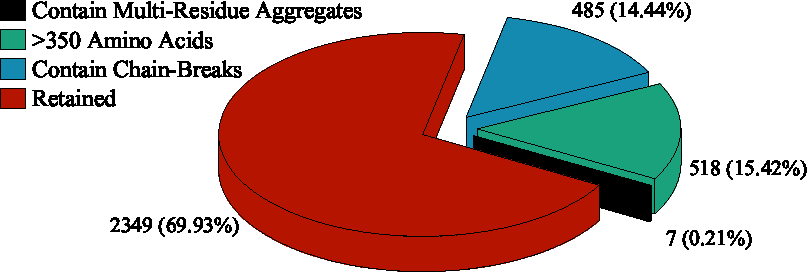
\includegraphics[width=0.8\textwidth]{./04-Database/CullPDBCounts/CullPDBCounts.pdf}
\caption{A summary of PDB structure culling for \thothdb.}
\label{fig:db:cull_pie}
\end{center}
\end{figure}

The final stage involved the structural refinement of the \finalchainlist\
using the functionality implemented in \pdbdb.
Missing \sidechain\ atoms were rebuilt using the highest propensity standard rotamer state which had minimal hard-sphere steric interaction with other defined atoms;  selected
from Richardson's penultimate rotamer library\cite{COMPCHEM:RICHARDSON}. Next, hydrogen atoms, which are missing from all \xray\ structures, were rebuilt using standard geometry as defined by \amber. 

As has been discussed in Section \ref{DB:NativeProbs} PDB structures sometimes contain atom positions in moderate steric overlap. In light of this, the structures were finally subjected to a short and gentle minimisation protocol
using the \pd\ simulation suite (section \ref{section:software:pd}). Thus,  any heavy steric clashes were removed, which could have caused simulations to fail or
behave unexpectedly. The gentle minimisation protocol used was extremely tolerant of any poor protein
geometry:\begin{enumerate} \isep
\item Minimise to a 0.1 \kcalmol\ energy gradient using \emph{only} the
standard \amberff\ bond, angle and torsion \forcefield\ terms. This will amend even extreme bond lengths without causing the minimisation to fail.
\item Minimise to a 0.1 \kcalmol\ energy gradient using the previous
\forcefield\ augmented with a soft-sphere steric \forcefield\ (figure \ref{fig:db:softvdw}).
This  results in atoms with heavy clashes moving gently away from each other until steric forces are satisfied. 
\item 
Finally, just 500 steps of minimisation were performed on the standard \ambergbsa\
\forcefield\ implemented in \pd. This ensured that electrostatic contacts were maintained whilst
the structure deviated little from its starting conformation.
\end{enumerate}
                   
                                 

\begin{figure}[hptb]
\begin{center}
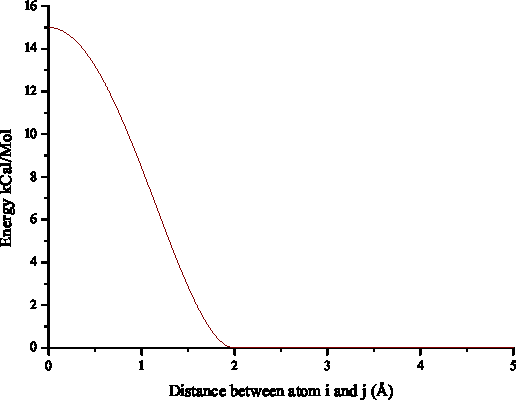
\includegraphics[width=0.5\textwidth]{04-Database/soft_sphere/potential.pdf}

\begin{equation}
E_\mathrm{softij}(h,x,d_\mathrm{ij},d'_\mathrm{ij}) = \left\{ \begin{array}{ll}
 h \left( 1.0 - \left(  d_\mathrm{ij}  / \left(  d'_\mathrm{ij} - x \right) \right) ^2 \right) ^2
  & \mbox{if $d_\mathrm{ij} < \left( d'_\mathrm{ij} - x \right)$ }\\
0 
  & \mbox{if $d_\mathrm{ij} \ge \left(d'_\mathrm{ij} - x \right)$ } \\
\end{array}
\right.
\end{equation}

\vspace{-0.5cm}

\begin{equation}
E_\mathrm{soft} = \sum^n_{i=1} \sum^n_{j=i+1} E_\mathrm{softij}
\end{equation}

\caption[The chosen soft-sphere potential]{The chosen soft-sphere potential,
where $h$ is the y-axis intercept which controls the hardness of the spheres
(default 15.0),
$d_\mathrm{ij}$ is the distance between atoms $i$ and $j$, $d'_\mathrm{ij}$ is the sum of their VDW radii (3.0 for the graph) and finally $x$ is an empirical  overlap tolerance
(default 1.0\AA). The calculation is summed for all atoms ($1\to n$) against
each atom with a higher numerical index.}
\label{fig:db:softvdw}
\end{center}
\end{figure}

As the minimisations were short, the minimised structures show a small all-atom \crms\ to the native structure, but some show a very significant difference in energy (figure \ref{datbase:minim}). The final mean, median and maximum
heavy-atom cRMS values for the 2,349 structures were 0.43\AA, 0.43\AA\ and 0.85\AA\ respectively.

\begin{figure}[htbp]
\begin{center}

\subfigure[Structural deviation following the gentle minimisation protocol
in an arbitrary typical section of the protein 
surface. The native and minimised structures are the blue and magenta respectively. ]{
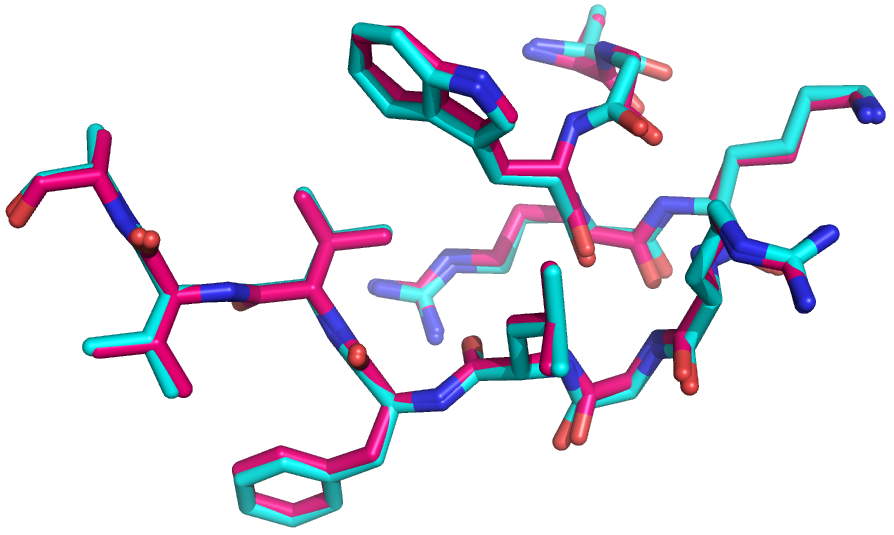
\includegraphics[width=0.75\textwidth]{./04-Database/img_protdb/MinStructureNoChange_zoom.png}}

\vspace{0.5cm}

\subfigure[The distribution of all heavy-atom \crms\ values between the native and \xray\ structures.]{
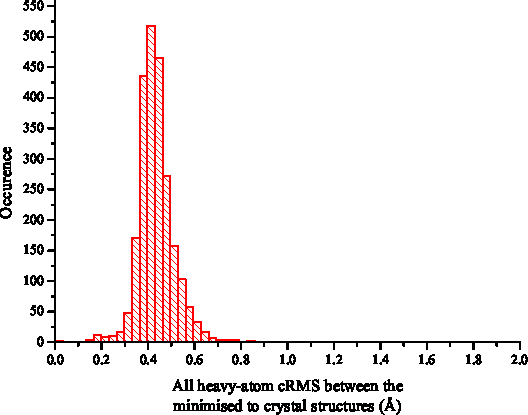
\includegraphics[width=0.75\textwidth]{04-Database/min_dev/MinimDeviation.pdf}}

\caption{Structural deviation following the gentle energy minimisation protocol.}
\label{datbase:minim}
\end{center}
\end{figure}


\subsection{Summary}

This section has described the process by which the PDB \jsubset\ for this
work was generated. For the task a specific application called \pdbdb\  was
developed which has the capabilities to both download the required PDB files
automatically and generate the required scripts to perform energy minimisation
using \pd. From this point, the resultant database of 2,349 high quality PDB structural files will be called \thothdb. 


\section{The Loop Database}
\label{section:intro:loop_db}

In true comparative modelling, a typical structurally variable region (SVR) or ``loop'' is usually defined as a region for which there is no discernible template sequence homology. In the majority of cases these regions  connect sections of regular secondary structure, but their exact bounds are dependent upon the method of sequence alignment,  the chosen template(s) and on the structural
alignment of those templates.
For calibration purposes in this study, the definition of a loop must be unambiguous.  Due to the close correlation between sections which span secondary
structures and those which are structurally variable between template structures, it was
decided that the loop definition of this work should be dictated by a solid secondary structure annotation algorithm.







\subsection{Secondary Structure Annotation}

In the past, secondary structure annotation was left to the structural biologist and was often inconsistent,
ambiguous and error prone. The advent of software applications for secondary structure annotation improved
this situation, however,
defining secondary structure from atomic coordinates alone is an inexact process due to differences in the exact definition used.
A study of three annotation methods exemplifies this by showing that on a non-redundant set of 154 proteins, all three methods agreed at only 63\% of residue positions\cite{NATIVE:Colloc1993}.
The choice of annotation method is, therefore, paramount as it is a cornerstone of the loop database definition
in this work.

\subsubsection{Annotation Methods}

\dssp \cite{NATIVE:DSSP}, or Dictionary for Secondary Structure Prediction, was released in 1983; implemented as a pattern recognition process of both geometric
and hydrogen bonded features and tested on a set of experimental coordinates. Overall, \dssp\ interprets \emph{cooperative} secondary structure from patterns of successive hydrogen bonded turns and bridges. Each residue is given one of a series of
characters  corresponding to its structural classification, shown
in table \ref{table:db:dssp}. \dssp\ is still seen today as one of the most consistent and accepted algorithms in secondary structure annotation and indeed bioinformatics as a whole; being cited in the scientific literature more than 1,000 times. However, alternatives do exist and were considered in this work. 

\begin{table}[hptb]
\begin{center}
\begin{tabular}{+c^l}
\toprule
\rowstyle{\bfseries}
     Code & Secondary Structure \\
\midrule
     H & \ahelix \\
     B & Isolated \be-bridge \\
     E & Extended strand, participates in \be-ladder \\
     G & 3\subscript{10}-helix \\
     I & $\pi$-helix\\
     T & Hydrogen bonded turn \\
     S & Bend \\
     -- & No structural annotation \\
\bottomrule
\end{tabular}
\caption{The secondary structure dictionary used by DSSP.}
\label{table:db:dssp}
\end{center}
\end{table}

In \dssp\ `E' is the annotation for a \bstrand. \dssp\ also allows \be-bulges to be assigned `E', allowing up to four residues on one side of sheet and one on the opposite side to be included in such a structure. The same is often not true of author annotations on the PDB \website\ or under other automated annotation methods. \be-bulges are, however, expected to be largely conserved between homologous structures.

\stride \cite{NATIVE:STRIDE} shows a number of similarities to \dssp\, but has a greater emphasis on backbone
torsions resulting in the inclusion of more residues at the termini of secondary structures.
\stride\ also adds an additional term in the expression of hydrogen bond energy,
which attempts to ensure planarity of the bond whilst allowing longer bonds to be included. Compared to \dssp, \stride\ tends to provide slightly
longer secondary structure annotations, although when compared pairwise, \dssp\ and \stride\ agree for approximately 95\% of residues\cite{NATIVE:Cuff1999}.

Part of the same method-family as \dssp\ and \stride\ is \secstr \cite{NATIVE::SECSTR}, which was developed
specifically to enhance the detection of $\pi$-helices. Unsurprisingly the
method therefore succeeds in categorising  additional structures to be $\pi$-helices when compared to \dssp. 

The method \define \cite{NATIVE:DEFINE} uses the distance separation between \ca\ atoms, variable between structure types, as its criterion for annotation. \define, however, has been shown to over-accommodate backbone distortion and therefore result in over-assignment of regular secondary structure. As a consequence \define\ assigns more than twice as many \bstrands\ of length four than most other methods\cite{NATIVE:Colloc1993}. \psea\ also relies solely on \ca\ coordinates and distance and angle criteria between
them\cite{NATIVE:PSEA}, but has been shown to largely agree with \stride \cite{NATIVE:KAKSI}.

\pcurve \cite{NATIVE:PCurve} is a third method type  which calculates
annotations using parameters like the tilt and roll between peptide planes. \pcurve\ also has a tendency to assign overly long elements of regular secondary structure. \xtlsstr\cite{NATIVE:XTLSSTR} analyses amide-amide interactions in an attempt to reproduce the same secondary structure annotations as would be derived by human visual inspection. \votap\cite{NATIVE:VOTAP} utilises Voronoi tessellation to produce contact matrices which are then used for annotation. 

Finally, \kaksi\cite{NATIVE:KAKSI}, one of the most recent additions to the field, uses both \ca\ distances and \phipsi\ angles during annotation, paying special attention to kink-detection in helices. Uniquely,
as annotation is sensitive to experimental determination method and resolution,
annotation parameters can be chosen dependent on the these properties. \kaksi\ was often shown to give several short secondary structures annotations with short breaks as opposed to a single large annotation. This generally results in fewer helix kinks and shorter more regular  secondary structures, which was an aim for the work.




\subsubsection{Structural Considerations for Annotation}


Residue geometry and hydrogen bonding patterns are less well defined towards the ends of regular secondary structures. That is to say, each amino acid still has similar backbone torsional angles, but those residues at either end of the structure often no longer exhibit hydrogen bonds.
This in turn means that, as sequence identity falls in comparative modelling, the ends of regular structures show significant variation  between multiple homologous templates.
In light of this, the \emph{under}-annotation of secondary structure length is preferable to over-annotation for the purposes of loop modelling calibration. On average,
this  yields longer loop definitions, but their use will result in a  fairer measure of the ability
of individual tools in real comparative modelling. 




\subsection{The Final Loop Definition}
\label{section:loopcriterion}

In summary, \dssp\ is still a solid bioinformatics standard and the most respected
annotation method currently available. Its annotations are typically shorter when compared to most other methods, however, this is desirable in this work
as the termini of secondary structures are the most structurally variable
in comparative modelling. \dssp\ also does not consider secondary structural
distortions like \be-bulges
to be separate structural types, which is again of benefit to this work as such structural distortions
are also expected to be  conserved. The use of DSSP should therefore ensure that the \dataset\ is especially representative of surface loops.
The exact loop definition used in this work is as follows:
\begin{enumerate}{} \isep
        \item  Using DSSP\cite{NATIVE:DSSP}, secondary structure annotation files were produced for non energy-minimised
PDB structures.        
        \item  ``Continuous'' regions of secondary structure are defined as a minimum of three residues of \bstrand\ (`E') or five residues of \ahelix\ (`H').
        \item  Loops are then defined as the connecting regions between these
continuous secondary structures, excluding the N and C-termini.       
        \item  Loops must be unbroken polypeptide in the available experimental data with all \sidechain\ heavy atoms
defined.
        \item  The standardised database itself does contain modified
residues which have been converted to standard residues. In contrast to this,
the loops themselves must \emph{not} have contained any modified residues
in the original PDB structure.

\end{enumerate}



\subsection{Loop Database Implementation}

As has been discussed, \thothdb\ represents a set of 2,349 high quality PDB and complementary \dssp\ files. The loop database itself is created on-the-fly by parsing the \dssp\ files as required. The inner details of the parsing process are encapsulated within a base-class called \textsl{DSSPTaskDirectory} which is present in the Methodology assembly of the \uobf\ as described in section
\ref{section:uobf:methodology}. Listing \ref{listing:db:dsspcode} shows that by deriving from this class, all the details of dealing
with this library of \dssp\ files and the subsequent extraction of information is abstracted away, leaving the user to deal solely with the problem at hand.


\lstset{language=CSharp}
\begin{lstlisting}[caption={Example code for \thothdb\ interaction.}, label=listing:db:dsspcode] 
// Derive a class from the base class `DSSPTaskDirectory' which
// embodies the abstract concept or parsing a folder of DSSP files
class Example_Thoth_DB_Client : DSSPTaskDirectory
{
    private static const int[] loopLengths = new int[] { 6, 7, 8, 9, 10, 11 };
    
    public void Execute()
    {
        // For each loop length we want to look at, run this loop...
        foreach (int loopLength in loopLengths)
        {
            ParsingFileIndex = 0; // reset IMPORTANT
            while (true)
            {    
                // *** The task we would like to perform ***
                SomeFunction( CurrentFile );

                // While we have further DSSP files, set CurrentFile to the next one...
                if (ParsingFileIndex < FileCount - 1) { ParsingFileIndex++; }
                else { break; } // Otherwise, break when we are done
            }
        }
    }
}

\end{lstlisting}

For each derived class, once the Execute() function has been added to the code, the object \textsl{CurrentFile} can be used. \textsl{CurrentFile} is an instance of the class \textsl{DSSPFile} and encodes all the
properties and information within a given \dssp\ output file. Listing \ref{listing:db:dsspoptions}
shows the three main function calls which can be made to \textsl{CurrentFile} dependent
upon the task at hand. For example, if the current task involves looking at loop structures, the function GetLoops() is called which returns all the loops
of the requested length(s) in the current \dssp\ file. These loops can then
be filtered and analysed as required by each individual task.

\lstset{language=CSharp}
\begin{lstlisting}[caption={Example code for DSSPFile class interaction.}, label=listing:db:dsspoptions] 
private void SomeFunction( DSSPFile currentFile )
{
    // Option 1) : GetResidues()
    // Perform analysis on individual resudues
    ResidueDef[] residues = CurrentFile.GetResidues();
    for (int j = 0; j < residues.Length; j++) 
              { DesiredFunction(residues[j]); } // act upon each residue


    // Option 2) : GetLoops()
    // Perform analysis on individual loops
    bool includeTerminii = false;
    bool validityFilter = true; // Remove unsatisfactory loops
    int loopLength = 8; // Include only 8-mers
    SegmentDef[] loops = CurrentFile.GetLoops(loopLength, includeTerminii, validityFilter);
    for (int j = 0; j < loops.Length; j++) 
              { DesiredFunction(loops[j]); } // act upon each loop


    // Option 3) : GetSecondaryStructures() 
    // Perform analysis on individual secondary structures 
    SegmentDef[] secStruc = CurrentFile.GetSecondaryStructures();
    for (int j = 0; j < loops.Length; j++) 
              { DesiredFunction(loops[j]); } // act upon each secondary structure
}
\end{lstlisting}

In this way, each given
task to be performed on the loop database can be easily encapsulated into a single
class. All of the analyses performed in chapter \ref{chapter:methods} are represented by
one or more of these classes which derive from \textsl{DSSPTaskDirectory} and utilise
the function call GetLoops().
 
\subsection{Loop Database Properties}
\label{section:loop_stats}

Following generation of the loop database in this work, structural features
were analysed and corresponding statistics generated. The difference in residue occurrence in all protein structure versus loop structure is shown in table \ref{table:database:propensity}, where in general the trends are as expected. The occurrence of hydrophobic residues is greatly reduced in surface
loops, whereas polar and charged residues are more prevalent. Proline, which
acts as a \mbox{helix-breaker} occurs 61\% more frequently in loop structure, whereas
helix-promoting alanine shows a 20\% reduction. Finally, due to its greater conformational freedom, glycine shows a 57\% increase in loop structure.
 
 

\begin{table}[htbp]
\begin{center}
\begin{tabular}[b]{+l^r^r^r^r^r^r}
\toprule
\rowstyle{\bfseries} 
 & \multicolumn{2}{c}{\textbf{All\ Structure}} & \multicolumn{2}{c}{\textbf{Loop\ Structure}} & Expected$^*$ & \% \\
\rowstyle{\bfseries} 
Residue / Class & Count & \multicolumn{1}{c}{\textbf{\%}} & Count & \multicolumn{1}{c}{\textbf{\%}} & \multicolumn{1}{c}{\textbf{Count}} & Difference  \\
\midrule
All Residues      & 733,048 & -      &  294,464   &  -      & -       & -                     \\
Charged           & 183,631 & 25.05  &  76,543    &  25.99  & 73,764  & 103.8   \\
Short Hydrophobic & 218,885 & 29.86  &  61,045    &  20.73  & 87,925  & \textcolor{red}{69.4} \\
Polar             & 183,629 & 25.05  &  80,642    &  27.39  & 73,763  & 109.3   \\
Bulky Aromatic    & 84,251  & 11.49  &  29,778    &  10.11  & 33,843  & \textcolor{red}{88.0} \\
Not Gly Or Pro    & 641,437 & 87.50  &  235,937   &  80.12  & 257,664 & \textcolor{red}{91.6} \\
Ala               & 61,446  & 8.38   &  19,849    &  6.74   & 24,682  & \textcolor{red}{80.4} \\
Arg               & 34,764  & 4.74   &  12,637    &  4.29   & 13,964  & \textcolor{red}{90.5} \\
Asn               & 32,510  & 4.43   &  17,887    &  6.07   & 13,059  & 137.0   \\
Asp               & 43,245  & 5.90   &  23,735    &  8.06   & 17,371  & 136.6   \\
Cys               & 10,653  & 1.45   &  3,861     &  1.31   & 4,279   & \textcolor{red}{90.2} \\
Gln               & 27,015  & 3.69   &  9,619     &  3.27   & 10,851  & \textcolor{red}{88.6} \\
Glu               & 46,337  & 6.32   &  16,312    &  5.54   & 18,613  & \textcolor{red}{87.6} \\
Gly               & 57,437  & 7.84   &  36,329    &  12.34  & 23,072  & 157.5   \\
His               & 16,921  & 2.31   &  7,377     &  2.51   & 6,797   & 108.5   \\
Ile               & 40,689  & 5.55   &  9,919     &  3.37   & 16,344  & \textcolor{red}{60.7} \\
Leu               & 63,696  & 8.69   &  17,987    &  6.11   & 25,586  & \textcolor{red}{70.3} \\
Lys               & 42,364  & 5.78   &  16,482    &  5.60   & 17,017  & \textcolor{red}{96.9} \\
Met               & 14,699  & 2.01   &  4,383     &  1.49   & 5,904   & \textcolor{red}{74.2} \\
Phe               & 29,478  & 4.02   &  9,643     &  3.27   & 11,841  & \textcolor{red}{81.4} \\
Pro               & 34,174  & 4.66   &  22,198    &  7.54   & 13,727  & 161.7   \\
Ser               & 44,551  & 6.08   &  22,238    &  7.55   & 17,896  & 124.3   \\
Thr               & 42,163  & 5.75   &  17,960    &  6.10   & 16,936  & 106.0   \\
Trp               & 11,115  & 1.52   &  3,681     &  1.25   & 4,464   & \textcolor{red}{82.5} \\
Tyr               & 26,737  & 3.65   &  9,077     &  3.08   & 10,740  & \textcolor{red}{84.5} \\
Val               & 53,054  & 7.24   &  13,290    &  4.51   & 21,311  & \textcolor{red}{62.4} \\
\bottomrule
\end{tabular}
\end{center}
\caption[\thothdb\ residue occurrence statistics]{\thothdb\ residue occurrence statistics: Observed and expected residue propensities are compared between all types of structure and loop structure only. 

$^*$The expected counts are theoretical extrapolations
created by multiplying the observed \%\ occurrence of each structural class by the total
number of loop total number of residues found in loop structures (294,464). Of course, as loop structure exhibits alternative residue propensities, the
observed occurrence is different. A reduction in residue propensity in loop regions is illustrated by
a red value in the
\% difference column.}
\label{table:database:propensity}
\end{table}




The distribution of loop lengths is shown in figure \ref{fig:Loop_DB_Hist},
where the majority of loops are under eight residues in length; although longer loops
of up to twelve residues are still very significant in number. Most of the ultra-long loops are highly convoluted regions containing only very small regions of secondary structure outside the definition used in this work. An example of this is shown
in figure \ref{fig:LDP_LongLoop} which depicts a \mer{56} surface region of 1AFWB where only two short regions of secondary structure exist and regular hydrogen bonding is minimal. The Ramachandran plot for this fragment shows some \mainchain\ torsional angles are on the outskirts of the normal Ramachandran regions.

\begin{figure}[htbp]
\begin{center}
    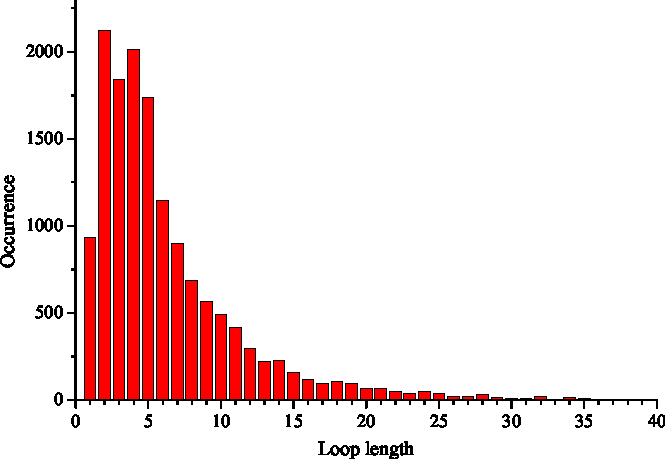
\includegraphics[width=0.8\textwidth]{./04-Database/img_loopdb/loop_length.pdf}
    \caption{Histogram showing the distribution of loop lengths resulting from the
chosen loop definition.}
    \label{fig:Loop_DB_Hist}
\end{center}
\end{figure}

\begin{figure}[htbp]
\begin{center}
  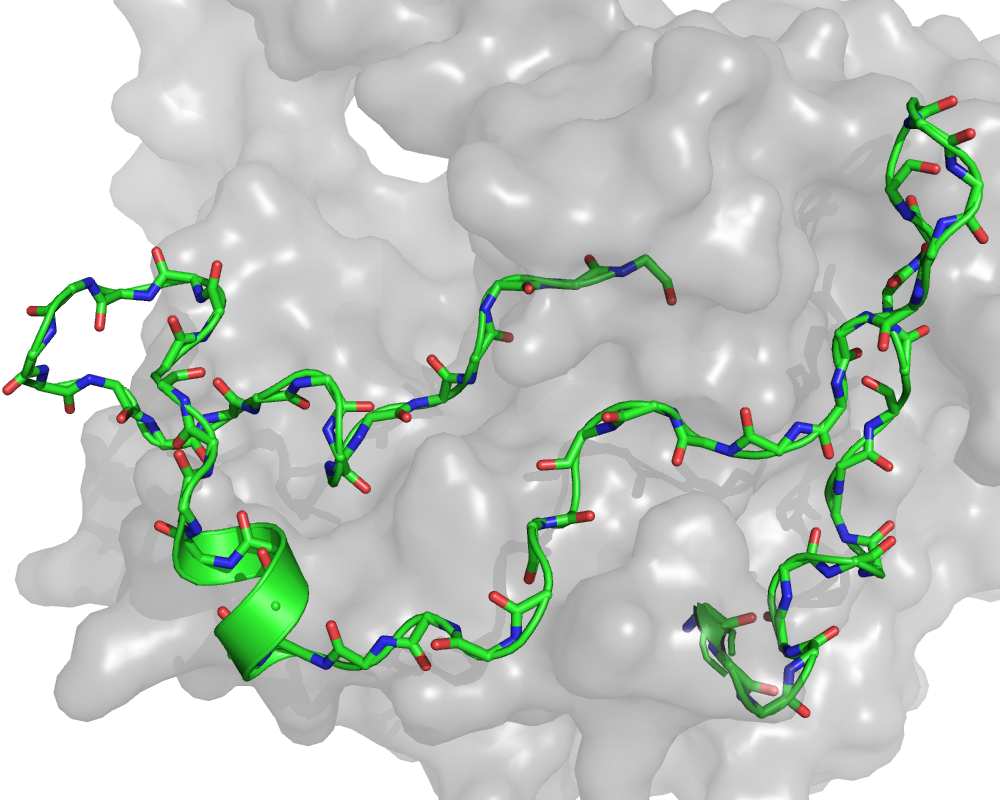
\includegraphics[width=0.8\textwidth]{./04-Database/img_loopdb/longloop.png}
  \newline                
  \mbox{ \small{DSSP Descriptor\cite{NATIVE:DSSP}}: \tiny{`TTTTTTTB--EE-TTS-EE-S-S---TT--HHHHTT---SSSTTT----TTSB---'}}
  \caption[A convoluted \mer{56} compound loop]{A convoluted \mer{56} compound loop taken from 1AFWB comprising of residues 221 to 276. Image created with \pymolV.}  
  \label{fig:LDP_LongLoop}
\end{center}
\end{figure}

This study focuses on medium to long  loops, which for the purposes
of this work will be defined
as those containing between 6 and 12 residues. As typical examples of 
this class of loop, some \mer{8} loops are shown
in figure \ref{fig:db:typicalloops}. The motifs, previously explained in section \ref{section:loop_structure}, are present in both  shorter length simple loops as well as parts of longer compound loops. The simplest class of loop is segments which span
two secondary structures that are distant in space, thus, a medium-length loop is required in order to span the gap; an example of this is shown in figure
\ref{fig:db:typicalloops}-a. These are usually packed tightly against the protein surface and often have hydrophobic residues inserted into the protein core
and solvent exposed hydrophilic residues.  In some cases a long loop is actually a heavily distorted secondary
structure, that was detected by \dssp\ as having no regular hydrogen bonding
pattern. Such a region is likely to have a poor sequence signal and therefore
would also be treated as a loop for the purposes of comparative modelling. An
example of this is in  figure \ref{fig:db:typicalloops}-b where the loop
folds across the back of two \bstrands\ in a large 8 strand \bsheet. This distorted loop
still shows some minor helical character, which if more defined would form
a standard strand-helix-strand motif. Finally, many longer loops are compound loops of the common motifs which characterise shorter loops. An example of this is shown in \mbox{figure \ref{fig:db:typicalloops}-c,} which is composed of a small helical region and a structure that resembles a \be-turn.



\begin{figure}[hptb]
  \begin{center}
  
            \subfigure[\mer{8} loop in 1O5XA from residue 29.]{\scalebox{0.54}{
            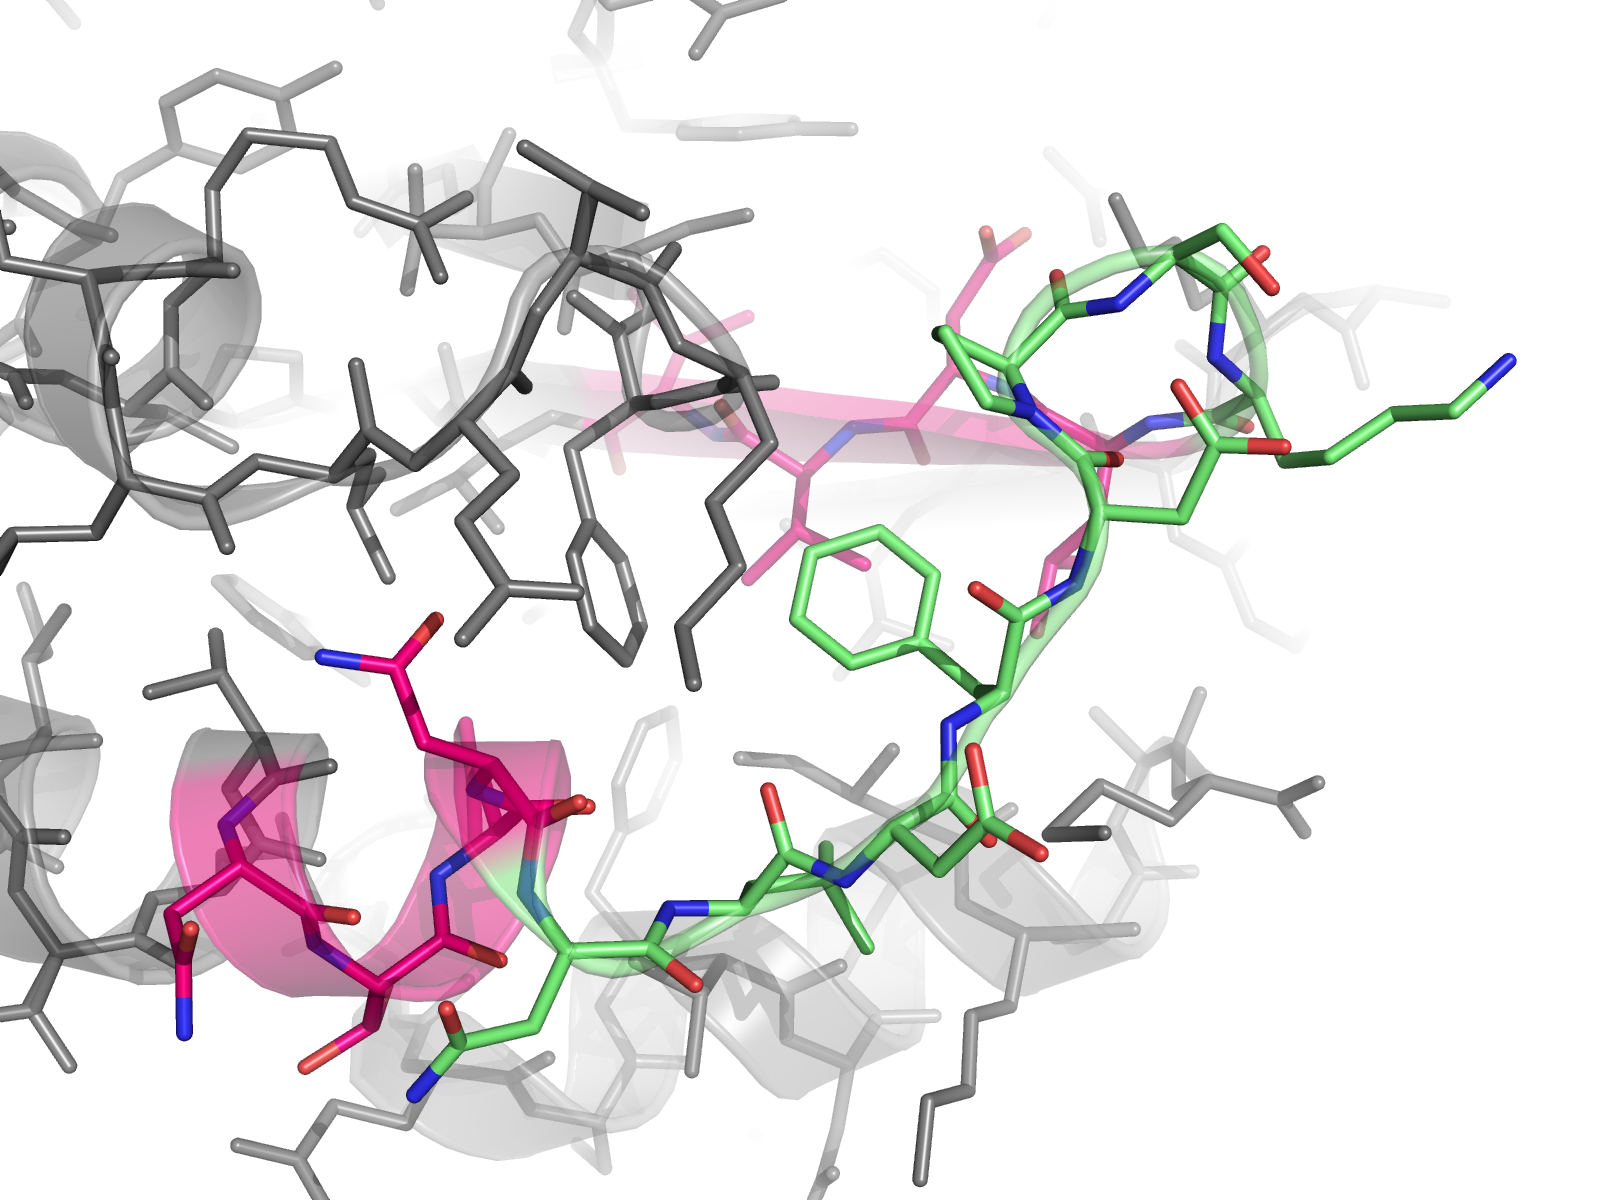
\includegraphics[width=1.0\textwidth]{04-Database/allowed/strand-helix.png}
            }}
            
           
            \subfigure[A typical loop formed within a distorted super-secondary structure motif. \mer{8} loop in 1OOEA from residue 35.]{\scalebox{0.54}{
            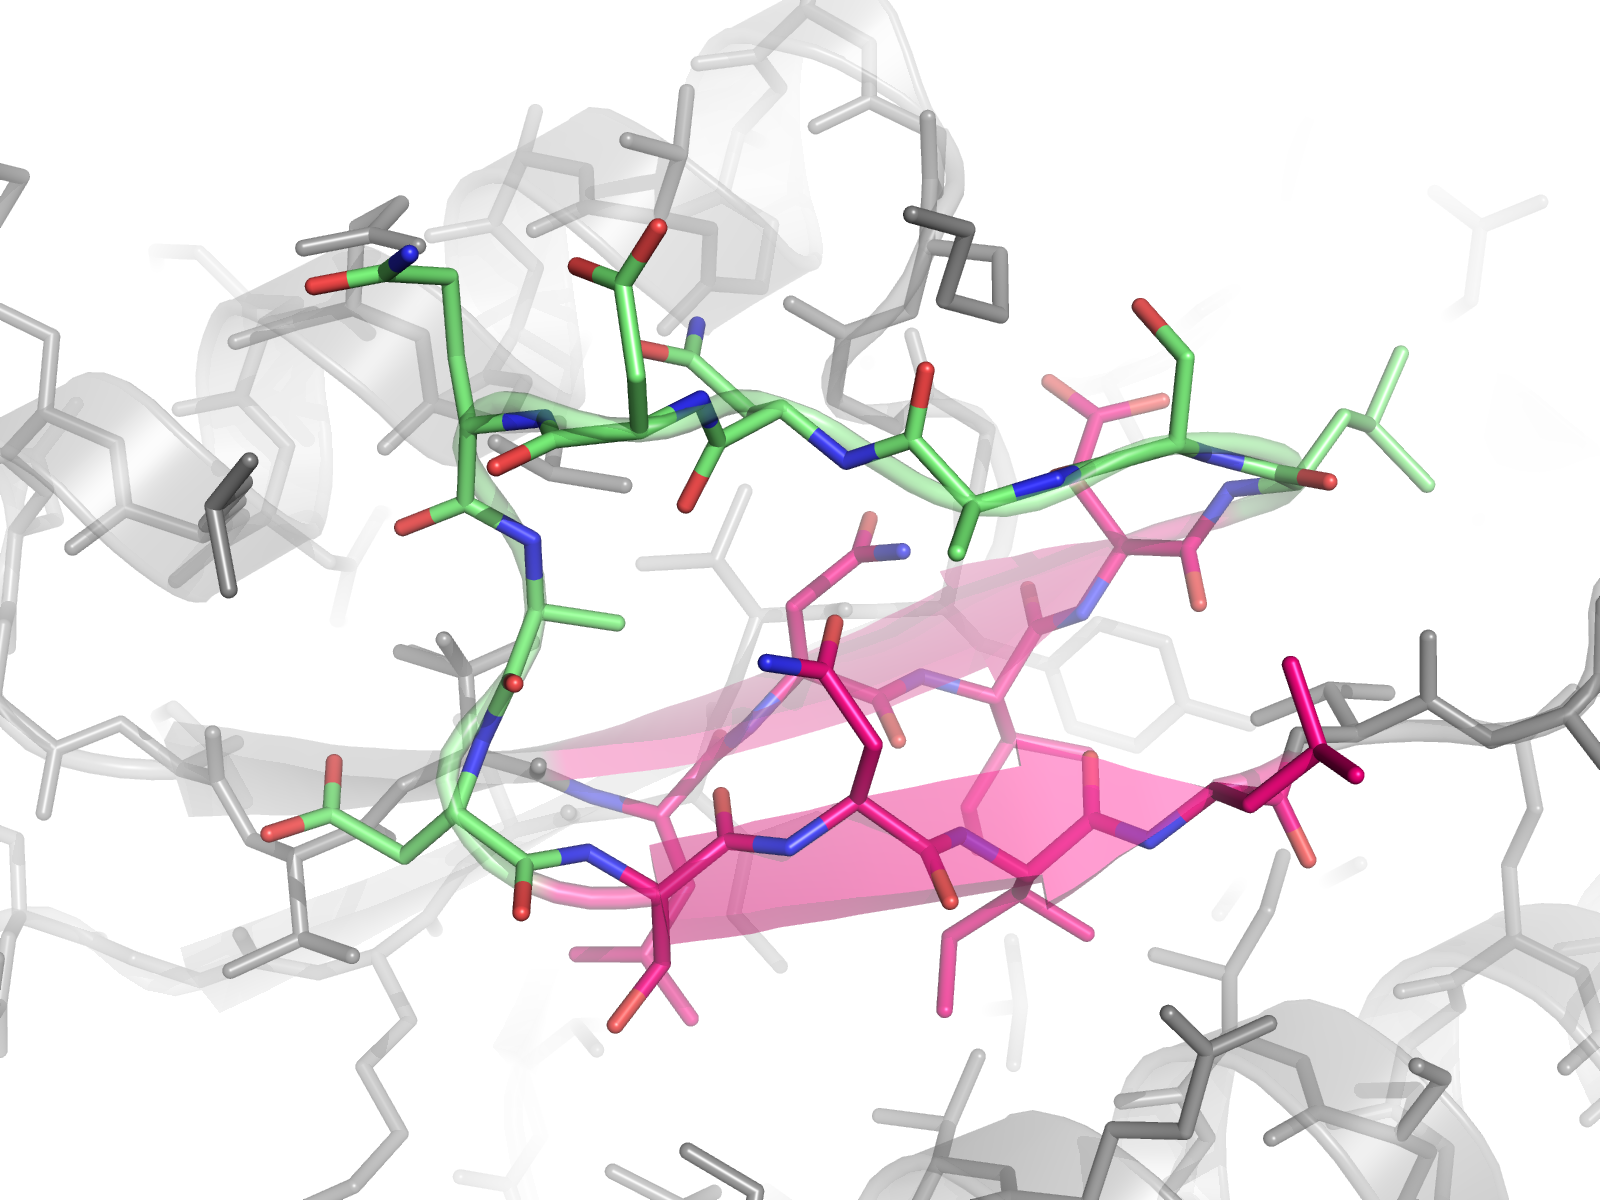
\includegraphics[width=1.0\textwidth]{04-Database/allowed/surface.png}
            }}
            
            \subfigure[A typical compound loop. \mer{8} loop in 1PFBA from residue 48.]{\scalebox{0.54}{
            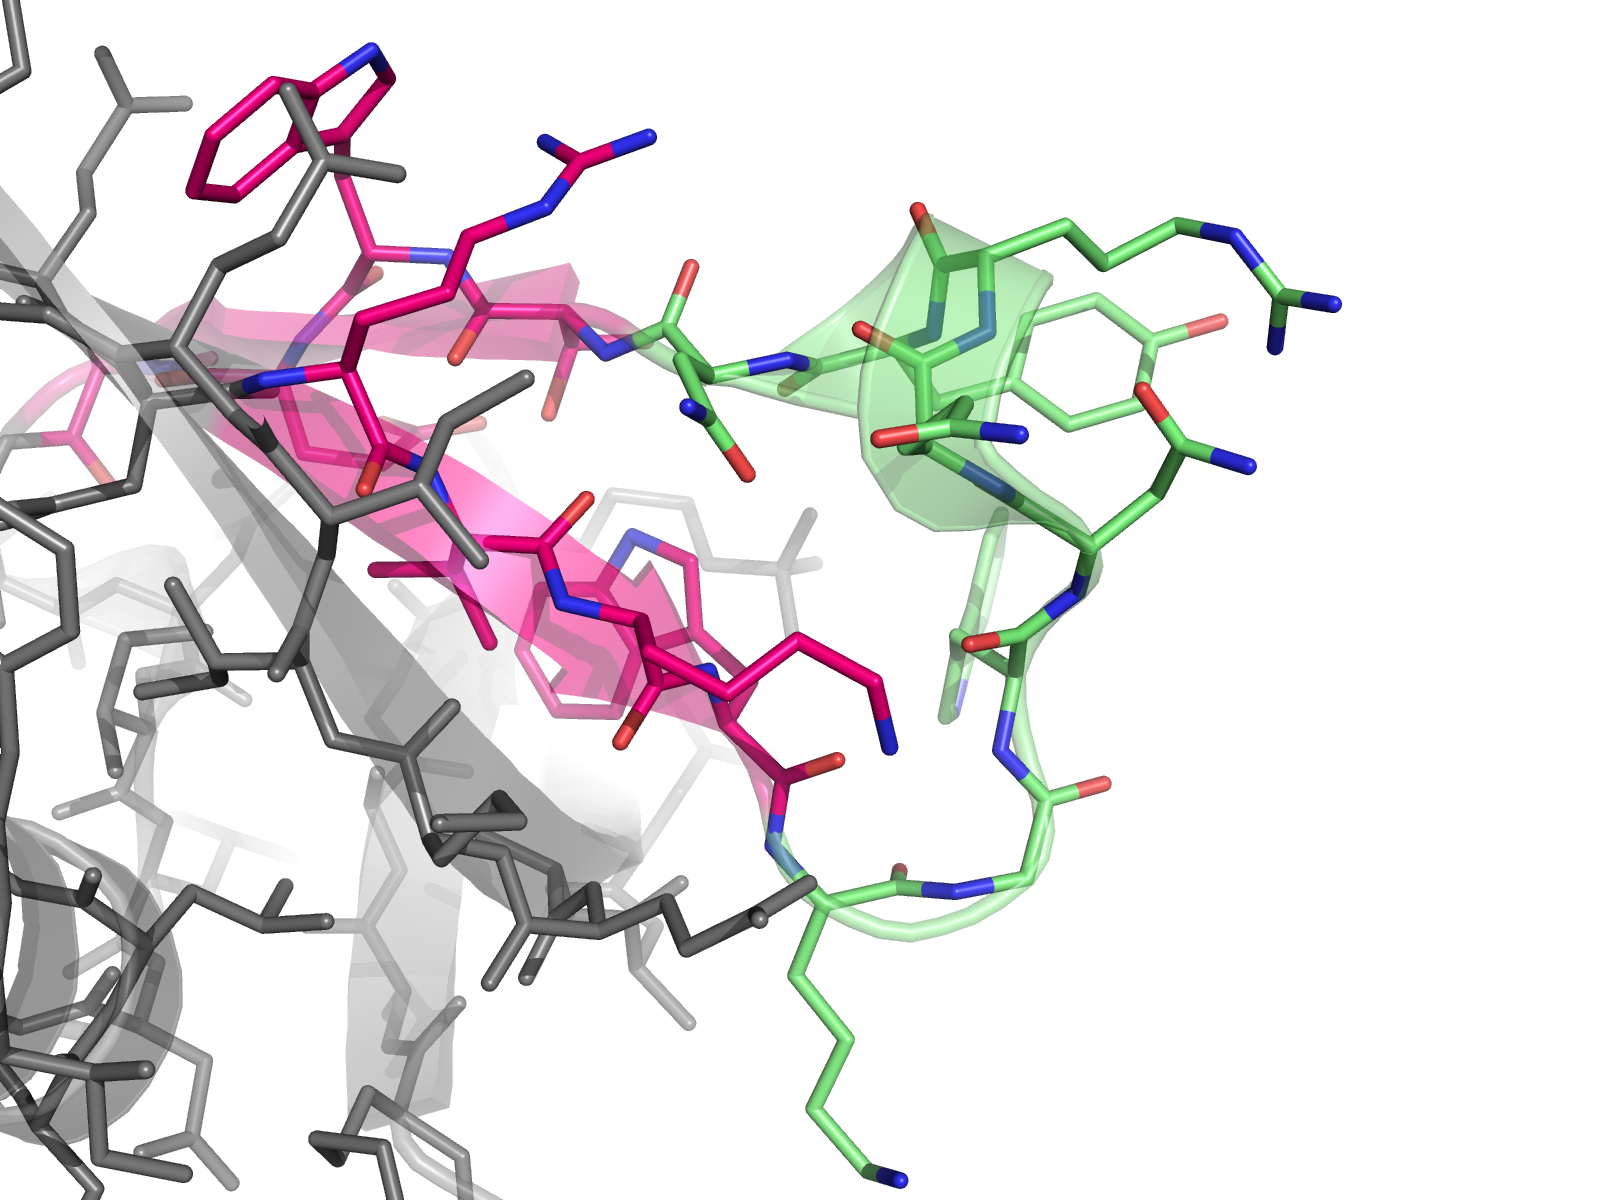
\includegraphics[width=1.0\textwidth]{04-Database/allowed/compound.png}
            }}
 
\caption[Typical medium to long range loops]{Typical medium to long length loops. 8-mers were chosen to illustrate the gross structural trends found
in this approximate size of  loop.
The loop and secondary structure anchors are shown in green and magenta respectively.
Images created with \pymolV.}

\label{fig:db:typicalloops}

\end{center}
\end{figure}







Importantly, table \ref{table:db:disallowedloop} shows that for longer loops the fraction 
of loops containing residues within
the disallowed regions of Ramachandran space increases several fold. Examples
of such loops are shown in figure \ref{fig:db:disallowedloop}. The fact that
up to 13.5\% of medium to long length loops have residues which populate these
regions of Ramachandran space (table \ref{table:db:disallowedloop}) has implications for the process of modelling
loops, specifically the scope of the conformational search.



\begin{table}[hp]
\begin{center}
\begin{tabular}{+c^c^c^c^c^c^c^c}
\toprule
  \multicolumn{2}{c}{\textbf{Loop}} & \multicolumn{6}{c}{\textbf{\% with Disallowed Angle}}\\

\rowstyle{\bfseries}
Length & Count  & I     & II    & III   & IV    & V    &  Any  \\
  
   \midrule
   0   &  321   &  0.0  &  0.0  &  0.0  &  0.0  &  0.0 &  0.0  \\
   1   &  930   &  0.4  &  3.1  &  0.2  &  0.1  &  0.0 &  3.9  \\
   2   &  2116  &  0.6  &  2.8  &  0.4  &  0.0  &  0.0 &  4.0  \\
   3   &  1817  &  1.8  &  0.8  &  0.6  &  0.0  &  0.1 &  3.2  \\
   4   &  2001  &  0.7  &  0.3  &  0.7  &  0.0  &  0.0 &  1.8  \\
   5   &  1730  &  1.9  &  1.1  &  0.7  &  0.6  &  0.1 &  4.3  \\
   \midrule
   6   &  1140  &  1.6  &  1.7  &  0.6  &  0.4  &  0.2 &  4.3  \\
   7   &  895   &  1.6  &  1.0  &  0.8  &  0.3  &  0.1 &  3.8  \\
   8   &  683   &  2.9  &  1.8  &  1.3  &  0.0  &  0.0 &  6.0  \\
   9   &  565   &  2.8  &  1.6  &  0.4  &  0.2  &  0.0 &  5.0  \\
   10  &  488   &  2.3  &  2.5  &  2.3  &  0.2  &  0.0 &  7.0  \\
   11  &  412   &  5.3  &  2.7  &  1.2  &  0.7  &  0.5 &  10.2 \\
   12  &  296   &  6.8  &  4.1  &  3.0  &  0.3  &  0.7 &  13.5 \\
   \midrule
   13  &  213   &  3.3  &  3.8  &  1.9  &  1.4  &  0.5 &  10.3 \\
   14  &  220   &  3.2  &  1.4  &  1.4  &  0.0  &  0.0 &  5.9  \\
   15  &  158   &  3.8  &  1.3  &  1.9  &  0.6  &  0.0 &  7.6  \\
   16  &  117   &  3.4  &  1.7  &  0.9  &  1.7  &  0.0 &  7.7  \\
   17  &  98    &  7.1  &  3.1  &  0.0  &  0.0  &  0.0 &  10.2 \\
   18  &  103   &  3.9  &  1.0  &  1.0  &  0.0  &  0.0 &  5.8  \\
   19  &  95    &  6.3  &  2.1  &  3.2  &  0.0  &  0.0 &  11.6 \\
   20  &  62    &  4.8  &  1.6  &  0.0  &  0.0  &  1.6 &  8.1  \\

\bottomrule
\end{tabular}
\caption[Loops containing residues in the disallowed Ramachandran regions.]{Loops containing residues in the disallowed Ramachandran regions. N.B. a zero length loop refers to a \ahelix\ directly joined to a \bstrand\ or visa-versa.}
\label{table:db:disallowedloop}
\end{center}
\end{table}





\begin{figure}[hptb]
  \begin{center}
  
    \mbox{  
    
            \subfigure[Ramachandran plot showing the five disallowed regions\cite{NATIVE:DISALLOWED}.]{\vspace{0.5cm}\scalebox{0.47}{
            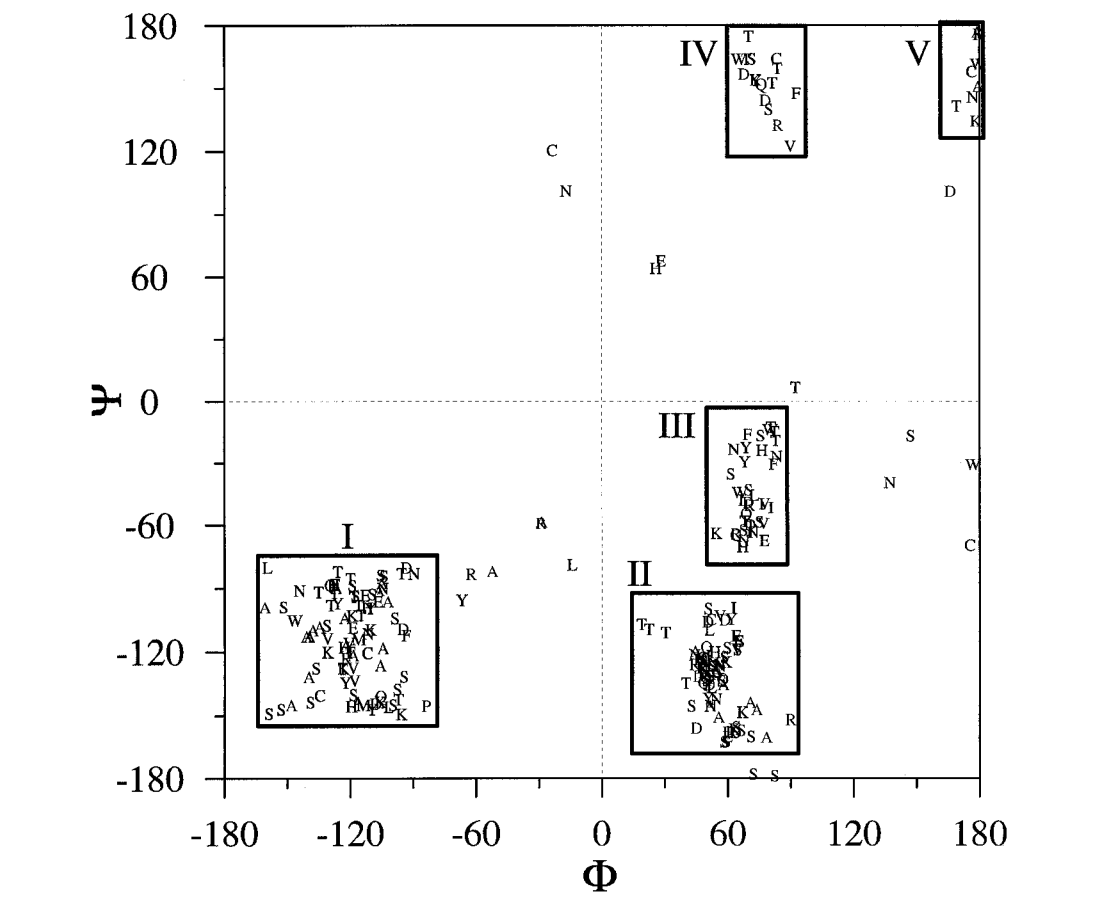
\includegraphics[width=0.884\textwidth]{04-Database/disallowed/disallowed.png}
            }}
            
            \quad
  
            \subfigure[Region I: A \mer{8} loop in 1SNNA from residue 21. Disallowed residue Lys-25 is stabilised by a close salt-bridge interaction.]{\scalebox{0.47}{
            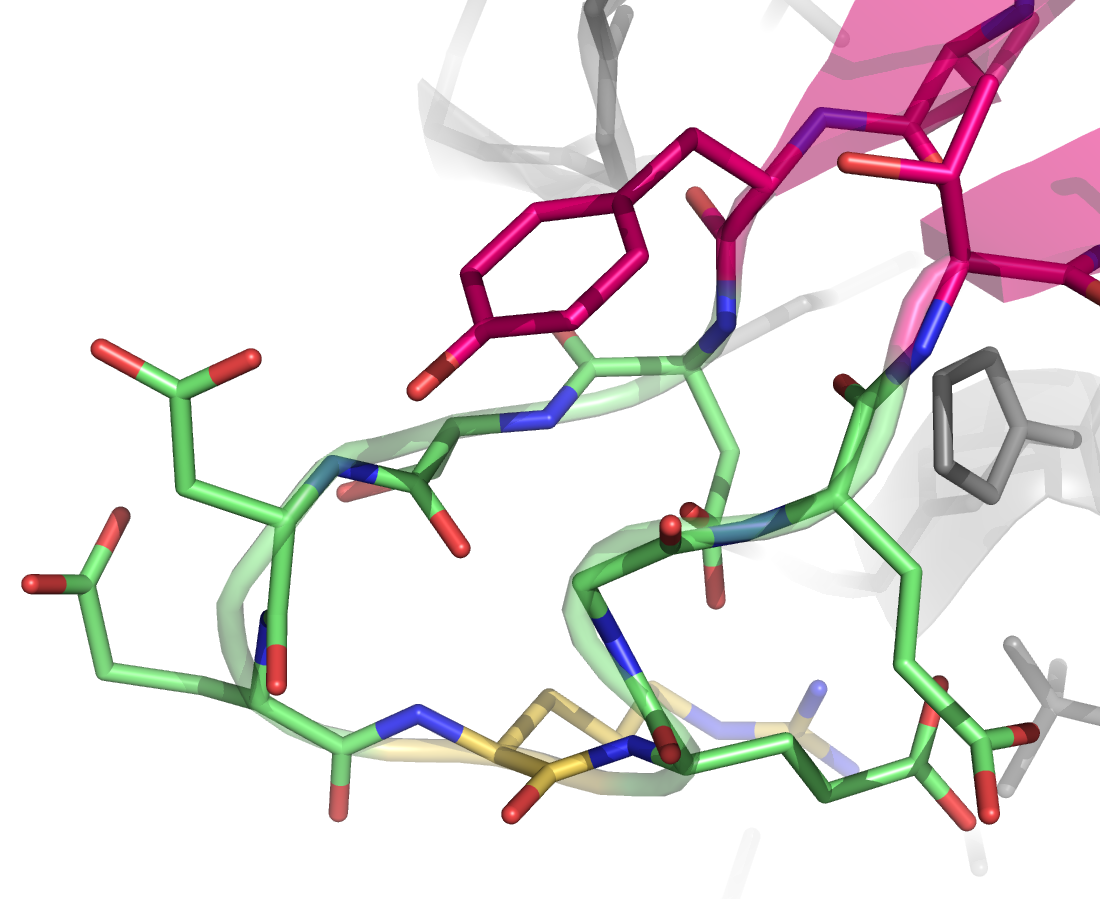
\includegraphics[width=0.884\textwidth]{04-Database/disallowed/region_1.png}
            }}
            
    } \mbox{ 
            
            \subfigure[Region II: A \mer{8} loop in 1JHJA from residue 83. A compound loop composed of a \be-turn and a very short helical region. Like in typical type II' beta turns, disallowed \mbox{Glu-87} is stabilised by an \mainchain\ \mbox{hydrogen bonding} interaction.]{\scalebox{0.47}{
            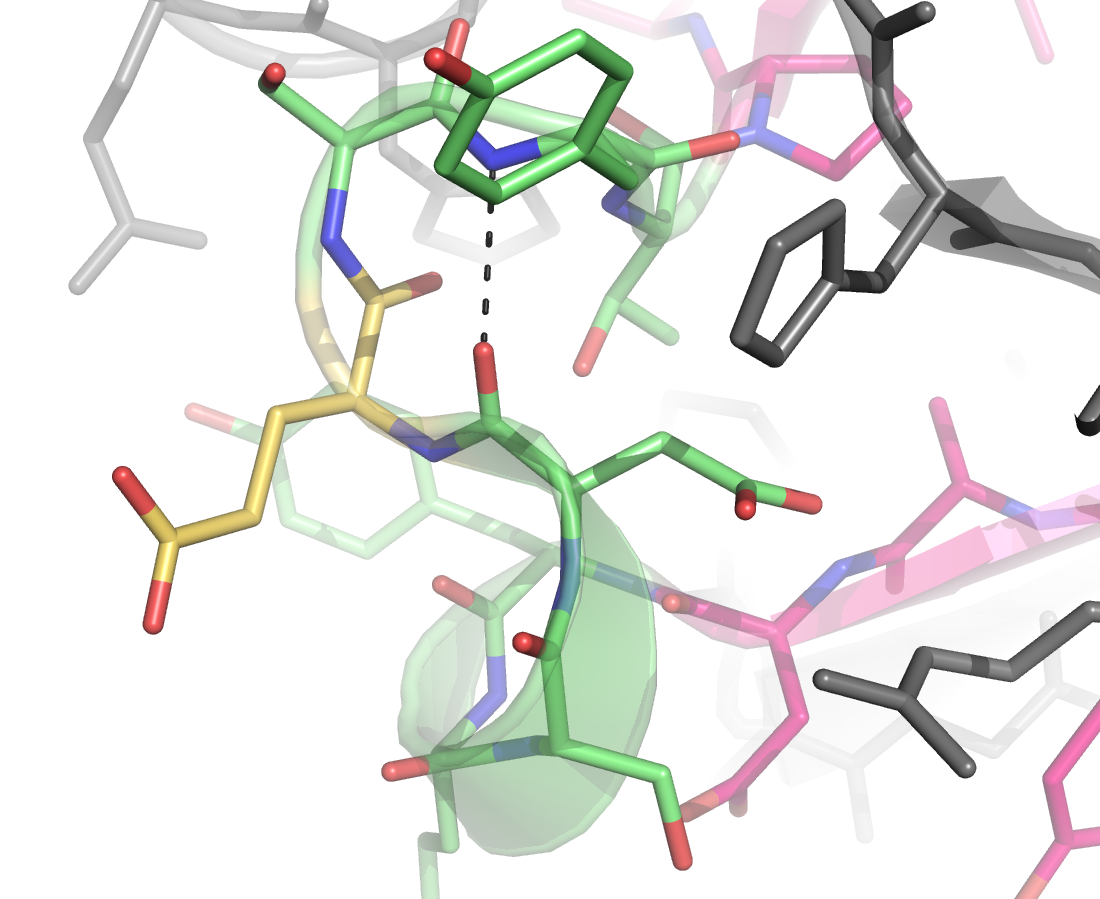
\includegraphics[width=0.884\textwidth]{04-Database/disallowed/region_2.png}
            }}
    
            \quad
    
            \subfigure[Region III: A \mer{8} loop in 1LZLA from residue 203. A particularly compact loop, where disallowed Leu-208 is packed tightly into the protein core.]{\scalebox{0.47}{
            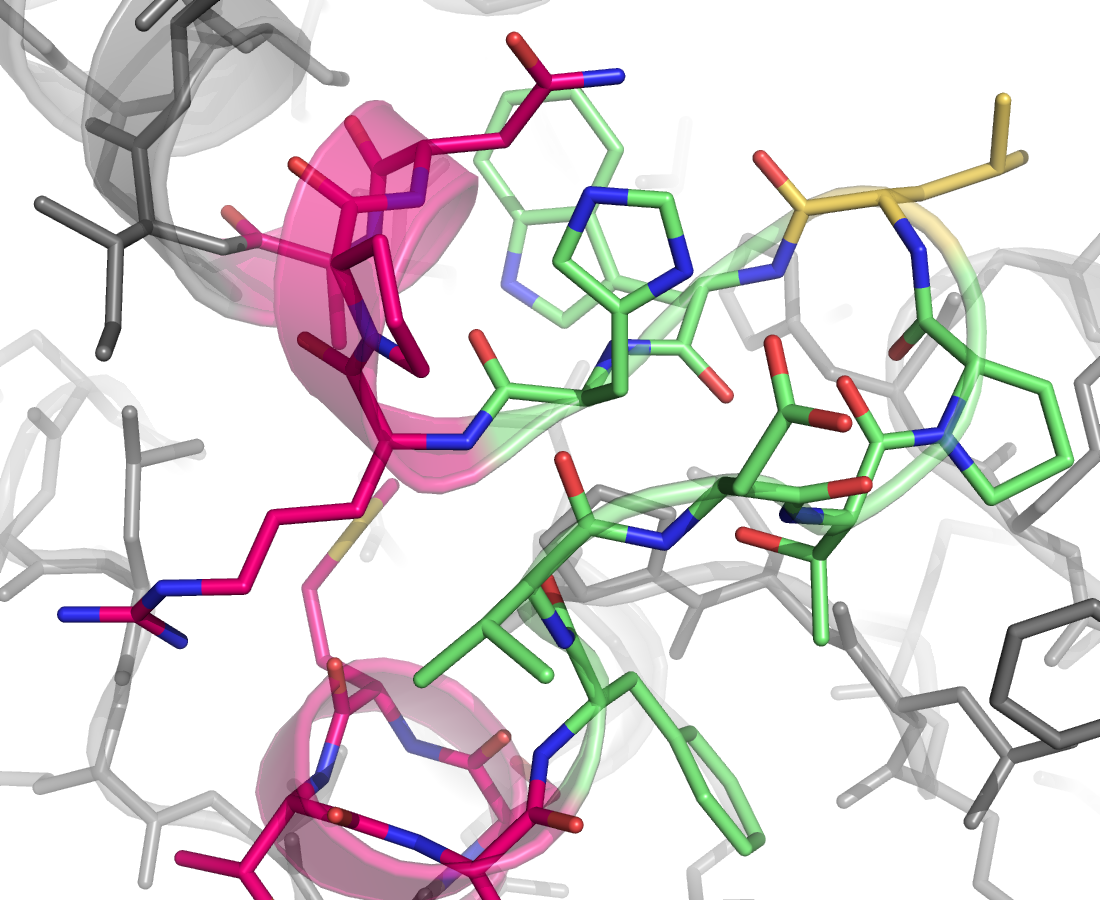
\includegraphics[width=0.884\textwidth]{04-Database/disallowed/region_3.png}
            }}
            
    } \mbox{
        
            \subfigure[Region IV: A \mer{7} loop in 2PTH\_ from residue 64. A compound loop involving a short helical region.]{\scalebox{0.47}{
            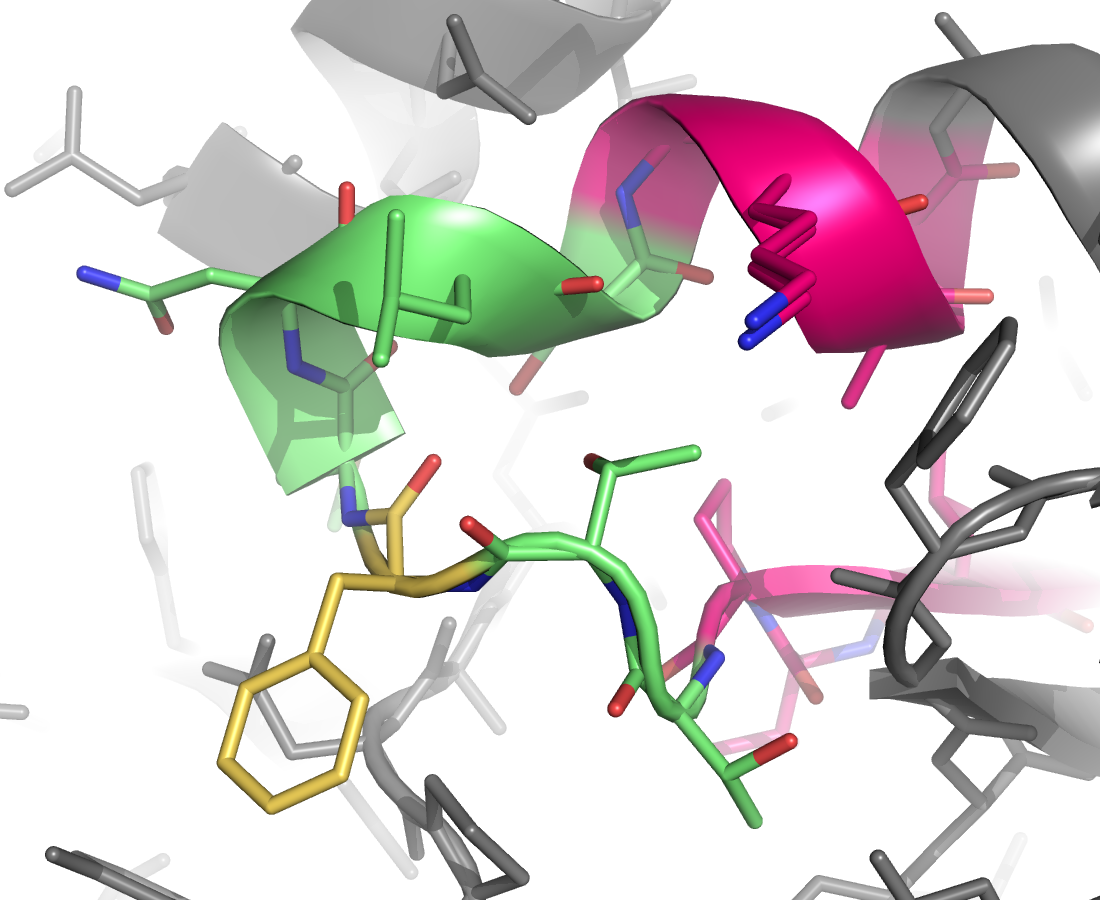
\includegraphics[width=0.884\textwidth]{04-Database/disallowed/region_4.png}
            }} 
    
            \quad
    
            \subfigure[Region V: A \mer{7} particularly extended loop in 1O6DA from residue 119. In this case, Ser-120 is stabilised by a \sidechain$\to$\mainchain\ hydrogen bond.]{\scalebox{0.47}{
            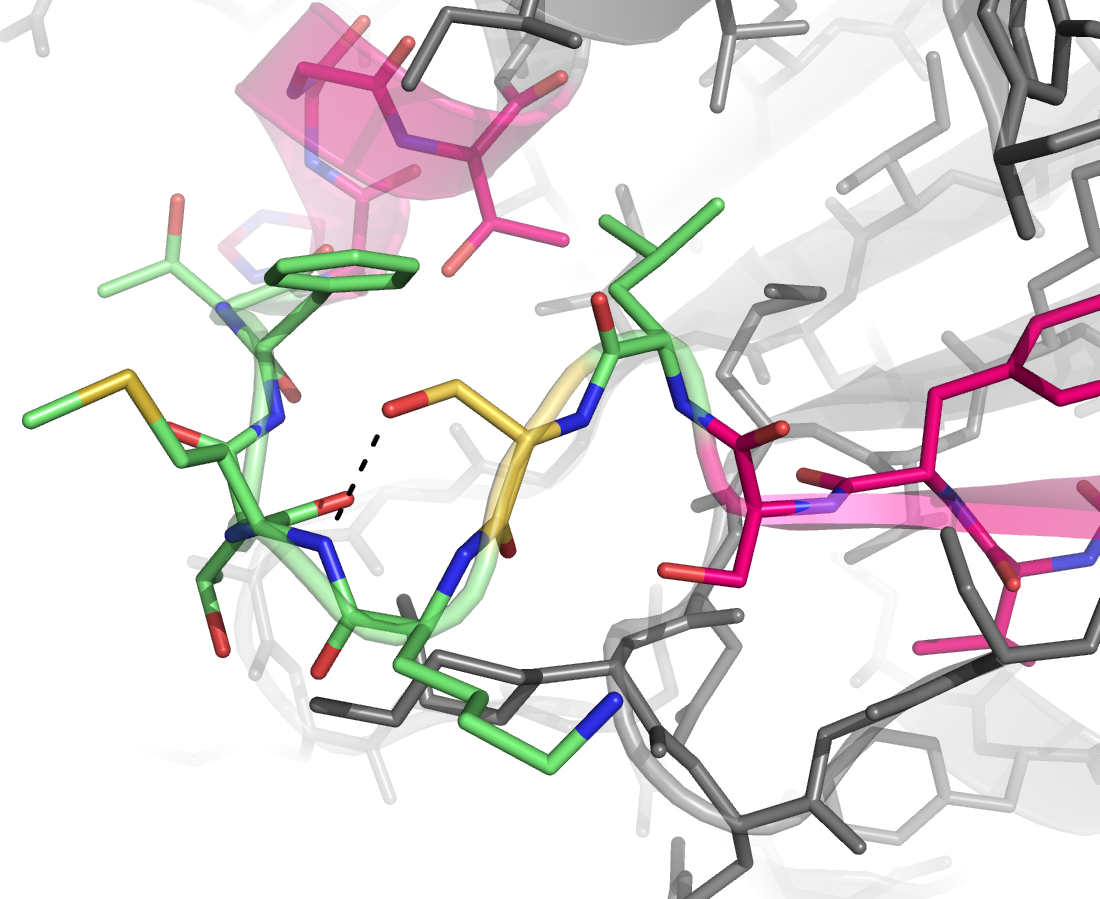
\includegraphics[width=0.884\textwidth]{04-Database/disallowed/region_5.png}
            }}}%
\caption[Loops with residues occupying disallowed regions of Ramachandran
    space]{Loops with residues occupying disallowed regions of Ramachandran
    space. For all images the disallowed residue, loop and anchor residues
    are in yellow, green and magenta respectively. Images created with \pymolV.}%
\label{fig:db:disallowedloop}
    
  \end{center}
\end{figure}







\subsection{Final Comments}

\subsubsection{Previous Loop Test Sets}

The most common benchmarks used in previous individual loop modelling calibrations are the test sets from Xiang et al.\cite{METHOD:Xia2002} and Fiser et al.\cite{METHOD:Fis2000}. These sets both used structures of $<$2.0\AA\ resolution,  a pairwise sequence identity cutoff of 20\% and 60\% respectively and contain loops of length 5$\to$12 and
1$\to$14 residues respectively. Fiser et al. chose 40 loops at random of each length with no more than one from each original PDB structure. By contrast Xiang et al. used all loops present within their smaller \dataset\ which contained 135 proteins derived from CulledPDB. The loop definitions used by these studies are similar to the definition developed during this work in that \dssp\ was used to define loop
boundaries. By contrast however, Fiser defines no prescribed lower limit on secondary structure length and Xiang uses any secondary structure annotation instead of only `H' and `E'.

 
It has been noted that the \mer{11} and \mer{12} residue loops in the Fiser \testset\ contain a high degree of secondary structure from the protein core\cite{METHOD:Plop},
although it is unclear why these would not have been filtered by their criteria. In any case these structures are inherently more appropriate for comprehensive building algorithms that utilise knowledge of either \ahelix\ packing or \bsheet\ strand register to build elements of the protein core. They are, therefore, less appropriate to loop modelling as bulk secondary structure prediction is not  required in high sequence-identity comparative modelling. As the loop selection definition
used in this work is derived from strict secondary structure annotation, such concerns are removed. Only very short regions of secondary structure remain, which should lie within the attainable scope of any viable loop modelling methodology.



The largest structural test set used in a method calibration prior to this study was 833 loops ranging from 4 to 12 residues in length\cite{METHOD:Plop}. In comparison to this, this study uses a database of unprecedented size, using all loops of between 6 and 11 residues in length, from the set of 2,349 extremely high-resolution structures described in section \ref{chapter:database:protein}. The exact counts are shown in table \ref{table:db:exactloopcount}. The software can generate loops of any user-defined length, however, the upper limit of 11 residues was chosen to in this work limit the duration of 
simulations with such a large test set and limited computational resources.
 Methods such as \plop\cite{METHOD:Plop} specify that on a 1.4\ghz\ AMD based PC, the maximum time for a \mer{12}
 was 160 hours. Even with more powerful processors available now, performing this test on the 4,183 test loops is unrealistic with current computational resources.


\begin{table}[hbtp]
\begin{center}
\begin{tabular}{+c^c}
\toprule
\rowstyle{\bfseries}
  Length & Count \\
\midrule
6     &  1,140 \\
7     &  895 \\
8     &  683 \\
9     &  565 \\
10    &  488 \\
11    &  412 \\
\midrule
Total &  4,183 \\
\bottomrule
\end{tabular}
\caption{Exact counts for the chosen range of loops derived for this work.}
\label{table:db:exactloopcount}
\end{center}
\end{table}


\subsubsection{The Chosen Loop Definition}

Within the loop definition chosen for this work, it is possible to obtain short sections of secondary structure within longer compound loops. These could be for example a short \ahelix\ packed against the protein surface or a short additional \bstrand\ in hydrogen bonding contact with a \be-sheet. Within a given set of structural templates, longer regions of secondary structure are very likely to be structurally conserved and possess a strong sequence signal. These would, therefore, be included as part of the rigid body in standard comparative
modelling studies. The converse is true of short secondary structure.


In light of this, it is assumed
that the loop definition used in this work is compatible with the types of loop found in comparative modelling tasks and will therefore result in a fair test set. Of course, some particularly long regions will be also found, however derived statistics obtained from the analysis of these irregular regions will nonetheless remain valid. Calibration of loop modelling can be performed on a subset of these loops of a range of suitable lengths. 




\section{Summary}
In summary, PDB culling servers were compared to find the most suitable for use in this study. \textsc{Pisces} was chosen because of its continuing support, regular updates, and enhanced feature set. \pdbdb, which utilises
the \uobf, was used to post-screen this \basechainlist. The relevant PDB files were downloaded, parsed, modified, filtered, rebuilt and then energy minimised
using \pd. This final \jsubset\
of 2,349 PDB files and complementary \dssp\ files will be referred to at \thothdb.

 From \thothdb, using the structural annotation output of \dssp\ as the basis for the loop definition,\ a representative set of medium to long length loops was defined for use in this study. Any loop database derived on-the-fly
will be referred to as \thothloopdb. Unless otherwise stated, the loops contained within
\thothloopdb\ are defined exclusively by the filtered structures in \thothdb\ and the
loop definition provided in \mbox{section \ref{section:loopcriterion}}.
